\setcounter{section}{6}
\setcounter{subsection}{0}

\section{Derivadas}

% ==============================================================================
% PARTE 1: ENUNCIADOS
% ==============================================================================

% ------------------------------------------------------------------------------
% 7.1. INTRODUÇÃO
% ------------------------------------------------------------------------------
\subsection{Introdução}
\textit{Esta subseção não possui exercícios.}

\clearpage

% ------------------------------------------------------------------------------
% 7.2. DERIVADA DE UMA FUNÇÃO
% ------------------------------------------------------------------------------
\subsection{Derivada de uma Função}

\defderivadaformal
\defretatangente
\deffuncaoderivavel

\begin{exercicio}[1]
\label{ex:7.2.1}
Seja $f(x) = x^2 + 1$. Calcule:
\begin{enumerate}[label=\alph*)]
    \item $f'(1)$
    \item $f'(0)$
    \item $f'(x)$
\end{enumerate}
\linkresolucao{7.2.1}
\end{exercicio}

\begin{exercicio}[2]
\label{ex:7.2.2}
Seja $f(x) = 2x$. Pensando geometricamente, qual o valor que você espera para $f'(p)$? Calcule $f'(p)$.
\linkresolucao{7.2.2}
\end{exercicio}

\begin{exercicio}[3]
\label{ex:7.2.3}
Seja $f(x) = 3x + 2$. Calcule:
\begin{enumerate}[label=\alph*)]
    \item $f'(2)$
    \item $f'(0)$
    \item $f'(x)$
\end{enumerate}
\linkresolucao{7.2.3}
\end{exercicio}

\begin{exercicio}[4]
\label{ex:7.2.4}
Calcule $f'(p)$, pela definição, sendo dados:
\begin{enumerate}[label=\alph*)]
    \item $f(x) = x^2 + x$ e $p = 1$
    \item $f(x) = \sqrt{x}$ e $p = 4$
    \item $f(x) = 5x - 3$ e $p = -3$
    \item $f(x) = \frac{1}{x}$ e $p = 1$
    \item $f(x) = \sqrt{x}$ e $p = 3$
    \item $f(x) = \frac{1}{\sqrt{x^2}}$ e $p = 2$
    \item $f(x) = 2x^3 - x^2$ e $p = 1$
    \item $f(x) = \sqrt[3]{x}$ e $p = 2$
\end{enumerate}
\linkresolucao{7.2.4}
\end{exercicio}

\begin{exercicio}[5]
\label{ex:7.2.5}
Determine a equação da reta tangente em $(p, f(p))$ sendo dados:
\begin{enumerate}[label=\alph*)]
    \item $f(x) = x^2$ e $p = 2$
    \item $f(x) = \frac{1}{x}$ e $p = 2$
    \item $f(x) = \sqrt{x}$ e $p = 9$
    \item $f(x) = x^2 - x$ e $p = 1$
\end{enumerate}
\linkresolucao{7.2.5}
\end{exercicio}

\begin{exercicio}[6]
\label{ex:7.2.6}
Calcule $f'(x)$, pela definição:
\begin{enumerate}[label=\alph*)]
    \item $f(x) = x^2 + x$
    \item $f(x) = 3x - 1$
    \item $f(x) = x^3$
    \item $f(x) = \frac{1}{x}$
    \item $f(x) = 5x$
    \item $f(x) = 10$
    \item $f(x) = \frac{x}{x + 1}$
    \item $f(x) = \frac{1}{x^2}$
\end{enumerate}
\linkresolucao{7.2.6}
\end{exercicio}

\begin{exercicio}[7]
\label{ex:7.2.7}
Dê exemplo (por meio de um gráfico) de uma função $f$, definida e derivável em $\R$, tal que $f'(1) = 0$.
\linkresolucao{7.2.7}
\end{exercicio}

\begin{exercicio}[8]
\label{ex:7.2.8}
Dê exemplo (por meio de um gráfico) de uma função $f$, definida e derivável em $\R$, tal que $f'(x) > 0$ para todo $x$.
\linkresolucao{7.2.8}
\end{exercicio}

\begin{exercicio}[9]
\label{ex:7.2.9}
Dê exemplo (por meio de um gráfico) de uma função $f$, definida e derivável em $\R$, tal que $f'(0) < f'(1)$.
\linkresolucao{7.2.9}
\end{exercicio}

\begin{exercicio}[10]
\label{ex:7.2.10}
Dê exemplo (por meio de um gráfico) de uma função $f$, definida e contínua em $\R$, tal que $f'(1)$ não exista.
\linkresolucao{7.2.10}
\end{exercicio}

\begin{exercicio}[11]
\label{ex:7.2.11}
Dê exemplo (por meio de um gráfico) de uma função $f$, definida e derivável em $\R$, tal que $f'(x) > 0$ para $x < 1$ e $f'(x) < 0$ para $x > 1$.
\linkresolucao{7.2.11}
\end{exercicio}

\begin{exercicio}[12]
\label{ex:7.2.12}
Dê exemplo (por meio de um gráfico) de uma função $f$, definida e derivável em $\R$, tal que $f'(x) > 0$ para $x < 0$, $f'(x) < 0$ para $0 < x < 2$ e $f'(x) > 0$ para $x > 2$.
\linkresolucao{7.2.12}
\end{exercicio}

\begin{exercicio}[13]
\label{ex:7.2.13}
Dê exemplo (por meio de um gráfico) de uma função $f$, definida e derivável em $\R$, tal que $f'(0) = 0$ e $f'(1) = 0$.
\linkresolucao{7.2.13}
\end{exercicio}

\begin{exercicio}[14]
\label{ex:7.2.14}
Mostre que a função
\[
g(x) = \begin{cases} 
2x + 1 & \text{se } x < 1 \\ 
-x + 4 & \text{se } x \ge 1 
\end{cases}
\]
não é derivável em $p = 1$. Esboce o gráfico de $g$.
\linkresolucao{7.2.14}
\end{exercicio}

\begin{exercicio}[15]
\label{ex:7.2.15}
Seja $g(x) = \begin{cases} x^2 + 2 & \text{se } x < 1 \\ 2x + 1 & \text{se } x \ge 1 \end{cases}$
\begin{enumerate}[label=\alph*)]
    \item Mostre que $g$ é derivável em $p = 1$ e calcule $g'(1)$.
    \item Esboce o gráfico de $g$.
\end{enumerate}
\linkresolucao{7.2.15}
\end{exercicio}

\begin{exercicio}[16]
\label{ex:7.2.16}
Seja $f(x) = \begin{cases} 2 & \text{se } x \ge 0 \\ x^2 + 2 & \text{se } x < 0 \end{cases}$
\begin{enumerate}[label=\alph*)]
    \item Esboce o gráfico de $f$.
    \item $f$ é derivável em $p = 0$? Em caso afirmativo, calcule $f'(0)$.
\end{enumerate}
\linkresolucao{7.2.16}
\end{exercicio}

\begin{exercicio}[17]
\label{ex:7.2.17}
Seja $g(x) = \begin{cases} x + 1 & \text{se } x < 1 \\ -x + 3 & \text{se } x \ge 1 \end{cases}$
\begin{enumerate}[label=\alph*)]
    \item Esboce o gráfico de $g$.
    \item $g$ é derivável em $p = 1$? Por quê?
\end{enumerate}
\linkresolucao{7.2.17}
\end{exercicio}

\begin{exercicio}[18]
\label{ex:7.2.18}
Construa uma função $f\colon \R \to \R$ que seja contínua em $\R$ e que seja derivável em todos os pontos, exceto em $-1$, $0$ e $1$.
\linkresolucao{7.2.18}
\end{exercicio}

\begin{exercicio}[19]
\label{ex:7.2.19}
Construa uma função $f\colon \R \to \R$ que seja contínua em $\R$ e derivável em todos os pontos, exceto nos números inteiros.
\linkresolucao{7.2.19}
\end{exercicio}

\clearpage

% ------------------------------------------------------------------------------
% 7.3. DERIVADAS DE x^n E \sqrt[n]{x}
% ------------------------------------------------------------------------------
\subsection{Derivadas de $x^n$ e $\sqrt[n]{x}$}

\begin{exercicio}[1]
\label{ex:7.3.1}
Seja $f(x) = x^5$. Calcule:
\begin{enumerate}[label=\alph*)]
    \item $f'(x)$
    \item $f'(0)$
    \item $f'(2)$
\end{enumerate}
\linkresolucao{7.3.1}
\end{exercicio}

\begin{exercicio}[2]
\label{ex:7.3.2}
Calcule $g'(x)$ sendo $g$ dada por:
\begin{enumerate}[label=\alph*)]
    \item $g(x) = x^6$
    \item $g(x) = x^{100}$
    \item $g(x) = \dfrac{1}{x}$
    \item $g(x) = x^2$
    \item $g(x) = \dfrac{1}{x^3}$
    \item $g(x) = \dfrac{1}{x^7}$
    \item $g(x) = x$
    \item $g(x) = x^{-3}$
\end{enumerate}
\linkresolucao{7.3.2}
\end{exercicio}

\begin{exercicio}[3]
\label{ex:7.3.3}
Determine a equação da reta tangente ao gráfico de $f(x) = \dfrac{1}{x}$ no ponto de abscissa 2. Esboce os gráficos de $f$ e da reta tangente.
\linkresolucao{7.3.3}
\end{exercicio}

\begin{exercicio}[4]
\label{ex:7.3.4}
Determine a equação da reta tangente ao gráfico de $f(x) = \dfrac{1}{x^2}$ no ponto de abscissa 1. Esboce os gráficos de $f$ e da reta tangente.
\linkresolucao{7.3.4}
\end{exercicio}

\begin{exercicio}[5]
\label{ex:7.3.5}
Seja $f(x) = \sqrt[5]{x}$. Calcule:
\begin{enumerate}[label=\alph*)]
    \item $f'(x)$
    \item $f'(1)$
    \item $f'(-32)$
\end{enumerate}
\linkresolucao{7.3.5}
\end{exercicio}

\begin{exercicio}[6]
\label{ex:7.3.6}
Calcule $g'(x)$, sendo $g$ dada por:
\begin{enumerate}[label=\alph*)]
    \item $g(x) = \sqrt[4]{x}$
    \item $g(x) = \sqrt[6]{x}$
    \item $g(x) = \sqrt[8]{x}$
    \item $g(x) = \sqrt[9]{x}$
\end{enumerate}
\linkresolucao{7.3.6}
\end{exercicio}

\begin{exercicio}[7]
\label{ex:7.3.7}
Determine a equação da reta tangente ao gráfico de $f(x) = \sqrt[3]{x}$ no ponto de abscissa 1. Esboce os gráficos de $f$ e da reta tangente.
\linkresolucao{7.3.7}
\end{exercicio}

\begin{exercicio}[8]
\label{ex:7.3.8}
Seja $r$ a reta tangente ao gráfico de $f(x) = \dfrac{1}{x}$ no ponto de abscissa $p$. Verifique que $r$ intercepta o eixo $x$ no ponto de abscissa $2p$.
\linkresolucao{7.3.8}
\end{exercicio}

\begin{exercicio}[9]
\label{ex:7.3.9}
Determine a reta que é tangente ao gráfico de $f(x) = x^2$ e paralela à reta $y = 4x + 2$.
\linkresolucao{7.3.9}
\end{exercicio}

\clearpage

% ------------------------------------------------------------------------------
% 7.4. DERIVADAS DE e^x E ln(x)
% ------------------------------------------------------------------------------
\subsection{Derivadas de $e^x$ e $\ln(x)$}

\begin{exercicio}[1]
\label{ex:7.4.1}
Determine a equação da reta tangente ao gráfico de $f(x) = e^x$ no ponto de abscissa 0.
\linkresolucao{7.4.1}
\end{exercicio}

\begin{exercicio}[2]
\label{ex:7.4.2}
Determine a equação da reta tangente ao gráfico de $f(x) = \ln x$ no ponto de abscissa 1. Esboce os gráficos de $f$ e da reta tangente.
\linkresolucao{7.4.2}
\end{exercicio}

\begin{exercicio}[3]
\label{ex:7.4.3}
Seja $f(x) = a^x$, em que $a > 0$ e $a \neq 1$ é um real dado. Mostre que $f'(x) = a^x \ln a$.
\linkresolucao{7.4.3}
\end{exercicio}

\begin{exercicio}[4]
\label{ex:7.4.4}
Calcule $f'(x)$:
\begin{enumerate}[label=\alph*)]
    \item $f(x) = 2^x$
    \item $f(x) = 5^x$
    \item $f(x) = \pi^x$
    \item $f(x) = e^x$
\end{enumerate}
\linkresolucao{7.4.4}
\end{exercicio}

\begin{exercicio}[5]
\label{ex:7.4.5}
Seja $g(x) = \log_a x$, em que $a > 0$ e $a \neq 1$ é constante. Mostre que $g'(x) = \dfrac{1}{x \ln a}$.
\linkresolucao{7.4.5}
\end{exercicio}

\begin{exercicio}[6]
\label{ex:7.4.6}
Calcule $g'(x)$:
\begin{enumerate}[label=\alph*)]
    \item $g(x) = \log_3 x$
    \item $g(x) = \log_5 x$
    \item $g(x) = \log_\pi x$
    \item $g(x) = \ln x$
\end{enumerate}
\linkresolucao{7.4.6}
\end{exercicio}

\clearpage

% ------------------------------------------------------------------------------
% 7.5. DERIVADAS DE FUNÇÕES TRIGONOMÉTRICAS
% ------------------------------------------------------------------------------
\subsection{Derivadas de Funções Trigonométricas}

\begin{exercicio}[1]
\label{ex:7.5.1}
Seja $f(x) = \sen x$. Calcule:
\begin{enumerate}[label=\alph*)]
    \item $f'(x)$
    \item $f'\!\left(\dfrac{\pi}{4}\right)$
\end{enumerate}
\linkresolucao{7.5.1}
\end{exercicio}

\begin{exercicio}[2]
\label{ex:7.5.2}
Determine a equação da reta tangente ao gráfico de $f(x) = \sen x$ no ponto de abscissa 0.
\linkresolucao{7.5.2}
\end{exercicio}

\begin{exercicio}[3]
\label{ex:7.5.3}
Seja $f(x) = \cos x$. Calcule:
\begin{enumerate}[label=\alph*)]
    \item $f'(x)$
    \item $f'(0)$
    \item $f'\!\left(\dfrac{\pi}{3}\right)$
    \item $f'\!\left(-\dfrac{\pi}{4}\right)$
\end{enumerate}
\linkresolucao{7.5.3}
\end{exercicio}

\begin{exercicio}[4]
\label{ex:7.5.4}
Calcule $f'(x)$ sendo:
\begin{enumerate}[label=\alph*)]
    \item $f(x) = \tg x$
    \item $f(x) = \sec x$
\end{enumerate}
\linkresolucao{7.5.4}
\end{exercicio}

\begin{exercicio}[5]
\label{ex:7.5.5}
Determine a equação da reta tangente ao gráfico de $f(x) = \tg x$ no ponto de abscissa 0.
\linkresolucao{7.5.5}
\end{exercicio}

\begin{exercicio}[6]
\label{ex:7.5.6}
Seja $f(x) = \cotg x$. Calcule:
\begin{enumerate}[label=\alph*)]
    \item $f'(x)$
    \item $f'\!\left(\dfrac{\pi}{4}\right)$
\end{enumerate}
\linkresolucao{7.5.6}
\end{exercicio}

\begin{exercicio}[7]
\label{ex:7.5.7}
Seja $g(x) = \cossec x$. Calcule:
\begin{enumerate}[label=\alph*)]
    \item $g'(x)$
    \item $g'\!\left(\dfrac{\pi}{4}\right)$
\end{enumerate}
\linkresolucao{7.5.7}
\end{exercicio}

\clearpage

% ------------------------------------------------------------------------------
% 7.6. DERIVABILIDADE E CONTINUIDADE
% ------------------------------------------------------------------------------
\subsection{Derivabilidade e Continuidade}

\begin{exercicio}[1]
\label{ex:7.6.1}
Seja $f(x) = \begin{cases} x + 1 & \text{se } x < 2 \\ 1 & \text{se } x \ge 2 \end{cases}$
\begin{enumerate}[label=\alph*)]
    \item $f$ é contínua em 2? Por quê?
    \item $f$ é derivável em 2? Por quê?
\end{enumerate}
\linkresolucao{7.6.1}
\end{exercicio}

\begin{exercicio}[2]
\label{ex:7.6.2}
Seja $f(x) = \begin{cases} x^2 & \text{se } x \le 0 \\ -x^2 & \text{se } x > 0 \end{cases}$
\begin{enumerate}[label=\alph*)]
    \item $f$ é derivável em 0? Justifique.
    \item $f$ é contínua em 0? Justifique.
\end{enumerate}
\linkresolucao{7.6.2}
\end{exercicio}

\begin{exercicio}[3]
\label{ex:7.6.3}
Seja $f(x) = \begin{cases} -x + 3 & \text{se } x < 3 \\ x - 3 & \text{se } x \ge 3 \end{cases}$
\begin{enumerate}[label=\alph*)]
    \item $f$ é derivável em 3? Justifique.
    \item $f$ é contínua em 3? Justifique.
\end{enumerate}
\linkresolucao{7.6.3}
\end{exercicio}

\clearpage

% ------------------------------------------------------------------------------
% 7.7. REGRAS DE DERIVAÇÃO
% ------------------------------------------------------------------------------
\subsection{Regras de Derivação}

\begin{exercicio}[1]
\label{ex:7.7.1}
Calcule $f'(x)$:
\begin{enumerate}[label=\alph*)]
    \item $f(x) = 3x^2 + 5$
    \item $f(x) = x^3 + x^2 + 1$
    \item $f(x) = 3x^3 - 2x^2 + 4$
    \item $f(x) = 3x + \sqrt{x}$
    \item $f(x) = 5 + 3x^{-2}$
    \item $f(x) = 2\sqrt[3]{x}$
    \item $f(x) = 3x + \dfrac{1}{x}$
    \item $f(x) = \dfrac{4}{x} + \dfrac{5}{x^2}$
    \item $f(x) = \dfrac{2}{3}x^3 + \dfrac{1}{4}x^2$
    \item $f(x) = \sqrt[3]{x} + \sqrt{x}$
    \item $f(x) = 2x + \dfrac{1}{x} + \dfrac{1}{x^2}$
    \item $f(x) = 6x^3 + \sqrt[3]{x}$
    \item $f(x) = 5x^4 + bx^3 + cx^2 + k$, em que $b$, $c$ e $k$ são constantes.
\end{enumerate}
\linkresolucao{7.7.1}
\end{exercicio}

\begin{exercicio}[2]
\label{ex:7.7.2}
Seja $g(x) = x^3 + \dfrac{1}{x}$. Determine a equação da reta tangente ao gráfico de $g$ no ponto $(1, g(1))$.
\linkresolucao{7.7.2}
\end{exercicio}

\begin{exercicio}[3]
\label{ex:7.7.3}
Seja $f(x) = x^2 + \dfrac{1}{x}$.
\begin{enumerate}[label=\alph*)]
    \item Determine o ponto do gráfico de $f$ em que a reta tangente, neste ponto, seja paralela ao eixo $x$.
    \item Esboce o gráfico de $f$.
\end{enumerate}
\linkresolucao{7.7.3}
\end{exercicio}

\begin{exercicio}[4]
\label{ex:7.7.4}
Seja $f(x) = x^3 + 3x^2 + 1$.
\begin{enumerate}[label=\alph*)]
    \item Estude o sinal de $f'(x)$.
    \item Calcule $\lim\limits_{x \to +\infty} f(x)$ e $\lim\limits_{x \to -\infty} f(x)$.
    \item Utilizando as informações acima, faça um esboço do gráfico de $f$.
\end{enumerate}
\linkresolucao{7.7.4}
\end{exercicio}

\begin{exercicio}[5]
\label{ex:7.7.5}
Mesmo exercício que o anterior, considerando a função $f(x) = x^3 + x^2 - 5x$.
\linkresolucao{7.7.5}
\end{exercicio}

\begin{exercicio}[6]
\label{ex:7.7.6}
Seja $f(x) = x^3 + 3x$.
\begin{enumerate}[label=\alph*)]
    \item Determine a equação da reta tangente ao gráfico de $f$ no ponto de abscissa 0.
    \item Estude o sinal de $f'(x)$.
    \item Esboce o gráfico de $f$.
\end{enumerate}
\linkresolucao{7.7.6}
\end{exercicio}

\begin{exercicio}[7]
\label{ex:7.7.7}
Calcule $F'(x)$ em que $F(x)$ é igual a:
\begin{enumerate}[label=\alph*)]
    \item $\dfrac{x}{x^2 + 1}$
    \item $\dfrac{x^2 - 1}{x + 1}$
    \item $\dfrac{3x^2 + 3}{5x - 3}$
    \item $\dfrac{\sqrt{x}}{x + 1}$
    \item $5x + \dfrac{x}{x - 1}$
    \item $\sqrt{x} + \dfrac{3}{x^3 + 2}$
    \item $\dfrac{\sqrt[3]{x} + x}{\sqrt{x}}$
    \item $\dfrac{x + \sqrt[4]{x}}{x^2 + 3}$
\end{enumerate}
\linkresolucao{7.7.7}
\end{exercicio}

\begin{exercicio}[8]
\label{ex:7.7.8}
Seja $g(x) = \dfrac{x}{x^2 + 1}$.
\begin{enumerate}[label=\alph*)]
    \item Determine os pontos do gráfico de $g$ em que as retas tangentes, nestes pontos, sejam paralelas ao eixo $x$.
    \item Estude o sinal de $g'(x)$.
    \item Calcule $\lim\limits_{x \to +\infty} g(x)$ e $\lim\limits_{x \to -\infty} g(x)$.
    \item Utilizando as informações acima, faça um esboço do gráfico de $g$.
\end{enumerate}
\linkresolucao{7.7.8}
\end{exercicio}

\begin{exercicio}[9]
\label{ex:7.7.9}
Calcule $f'(x)$ em que $f(x)$ é igual a:
\begin{enumerate}[label=\alph*)]
    \item $3x^2 + 5\cos x$
    \item $\dfrac{\cos x}{x^2 + 1}$
    \item $x\sen x$
    \item $x^2 \tg x$
    \item $\dfrac{x + 1}{\tg x}$
    \item $\dfrac{3}{\sen x + \cos x}$
    \item $\dfrac{\sec x}{3x + 2}$
    \item $\cos x + (x^2 + 1)\sen x$
    \item $\sqrt{x}\sec x$
    \item $3\cos x + 5\sec x$
    \item $x\cotg x$
    \item $4\sec x + \cotg x$
    \item $x^2 + 3x\tg x$
    \item $\dfrac{x^2 + 1}{\sec x}$
    \item $\dfrac{x + 1}{x\sen x}$
    \item $\dfrac{x}{\cossec x}$
    \item $(x^3 + \sqrt{x})\cossec x$
    \item $\dfrac{x + \sen x}{x - \cos x}$
\end{enumerate}
\linkresolucao{7.7.9}
\end{exercicio}

\begin{exercicio}[10]
\label{ex:7.7.10}
Seja $f(x) = x^2 \sen x + \cos x$. Calcule:
\begin{enumerate}[label=\alph*)]
    \item $f'(x)$
    \item $f'(0)$
    \item $f'(3a)$
    \item $f'(x^2)$
\end{enumerate}
\linkresolucao{7.7.10}
\end{exercicio}

\begin{exercicio}[11]
\label{ex:7.7.11}
Seja $f(x) = \sen x + \cos x$, $0 \le x \le 2\pi$.
\begin{enumerate}[label=\alph*)]
    \item Estude o sinal de $f'(x)$.
    \item Faça um esboço do gráfico de $f$.
\end{enumerate}
\linkresolucao{7.7.11}
\end{exercicio}

\begin{exercicio}[12]
\label{ex:7.7.12}
Calcule $f'(x)$:
\begin{enumerate}[label=\alph*)]
    \item $f(x) = x^2 e^x$
    \item $f(x) = 3x + 5\ln x$
    \item $f(x) = e^x \cos x$
    \item $f(x) = \dfrac{1 + e^x}{1 - e^x}$
    \item $f(x) = x^2 \ln x + 2e^x$
    \item $f(x) = \dfrac{x + 1}{x\ln x}$
    \item $f(x) = 4 + 5x^2 \ln x$
    \item $f(x) = \dfrac{e^x}{x^2 + 1}$
    \item $f(x) = \dfrac{\ln x}{x}$
    \item $f(x) = \dfrac{e^x}{x + 1}$
\end{enumerate}
\linkresolucao{7.7.12}
\end{exercicio}

\begin{exercicio}[13]
\label{ex:7.7.13}
Sejam $f$, $g$ e $h$ funções deriváveis. Verifique que:
\[
[f(x)g(x)h(x)]' = f'(x)g(x)h(x) + f(x)g'(x)h(x) + f(x)g(x)h'(x).
\]
\linkresolucao{7.7.13}
\end{exercicio}

\begin{exercicio}[14]
\label{ex:7.7.14}
Calcule $F'(x)$ sendo $F(x)$ igual a:
\begin{enumerate}[label=\alph*)]
    \item $x e^x \cos x$
    \item $x^2 (\cos x)(1 + \ln x)$
    \item $e^x \sen x \cos x$
    \item $(1 + \sqrt{x})e^x \tg x$
\end{enumerate}
\linkresolucao{7.7.14}
\end{exercicio}

\clearpage

% ------------------------------------------------------------------------------
% 7.8. FUNÇÃO DERIVADA E DERIVADAS DE ORDEM SUPERIOR
% ------------------------------------------------------------------------------
\subsection{Função Derivada e Derivadas de Ordem Superior}

\begin{exercicio}[1]
\label{ex:7.8.1}
Determine $f'$, $f''$ e $f'''$:
\begin{enumerate}[label=\alph*)]
    \item $f(x) = 4x^4 + 2x$
    \item $f(x) = \dfrac{1}{x}$
    \item $f(x) = 5x^2 - \dfrac{1}{x^3}$
    \item $f(x) = 3x^3 - 6x + 1$
    \item $f(x) = x|x|$
    \item $f(x) = \begin{cases} x^2 + 3x & \text{se } x \le 1 \\ 5x - 1 & \text{se } x > 1 \end{cases}$
\end{enumerate}
\linkresolucao{7.8.1}
\end{exercicio}

\begin{exercicio}[2]
\label{ex:7.8.2}
Esboce os gráficos de $f$, $f'$ e $f''$:
\begin{enumerate}[label=\alph*)]
    \item $f(x) = x^2 |x|$
    \item $f(x) = \begin{cases} x^2 + 3x & \text{se } x \le 1 \\ 5x - 1 & \text{se } x > 1 \end{cases}$
\end{enumerate}
\linkresolucao{7.8.2}
\end{exercicio}

\begin{exercicio}[3]
\label{ex:7.8.3}
Determine a derivada de ordem $n$:
\begin{enumerate}[label=\alph*)]
    \item $f(x) = e^x$
    \item $f(x) = \sen x$
    \item $f(x) = \cos x$
    \item $f(x) = \ln x$
\end{enumerate}
\linkresolucao{7.8.3}
\end{exercicio}

\clearpage

% ------------------------------------------------------------------------------
% 7.9. NOTAÇÕES PARA A DERIVADA
% ------------------------------------------------------------------------------
\subsection{Notações para a Derivada}

\begin{exercicio}[1]
\label{ex:7.9.1}
Calcule a derivada:
\begin{enumerate}[label=\alph*)]
    \item $y = 5x^3 + 6x - 1$
    \item $s = \sqrt[5]{t} + \dfrac{3}{t}$
    \item $x = \dfrac{t}{t + 1}$
    \item $y = t \cos t$
    \item $y = \dfrac{u + 1}{\ln u}$
    \item $x = t^3 e^t$
    \item $s = e^t \tg t$
    \item $y = \dfrac{x^3 + 1}{\sen x}$
    \item $y = \sqrt[3]{u} \sec u$
    \item $x = \dfrac{3}{t} + \dfrac{2}{t^2}$
    \item $x = e^t \cos t$
    \item $u = 5v^2 + \dfrac{3}{v^4}$
    \item $V = \dfrac{4}{3}\pi r^3$
    \item $E = \dfrac{1}{2}v^2$
    \item $E = \dfrac{1}{2}mv^2$, $m$ constante
    \item $U = \dfrac{a}{x^{12}} - \dfrac{b}{x^6}$, $a$ e $b$ constantes
\end{enumerate}
\linkresolucao{7.9.1}
\end{exercicio}

\begin{exercicio}[2]
\label{ex:7.9.2}
Seja $y = \dfrac{x^3}{x + \sqrt{x}}$. Calcule:
\begin{enumerate}[label=\alph*)]
    \item $\deriv{y}{x}$
    \item $\left.\deriv{y}{x}\right|_{x = 1}$
\end{enumerate}
\linkresolucao{7.9.2}
\end{exercicio}

\begin{exercicio}[3]
\label{ex:7.9.3}
Seja $y = t^2 x$, em que $x = x(t)$ é uma função derivável. Calcule $\left.\deriv{y}{t}\right|_{t = 1}$ supondo $\left.\deriv{x}{t}\right|_{t = 1} = 2$ e $x = 3$ para $t = 1$ (isto é, $x(1) = 3$).
\linkresolucao{7.9.3}
\end{exercicio}

\begin{exercicio}[4]
\label{ex:7.9.4}
Considere a função $y = xt^3$, na qual $x = x(t)$ é uma função derivável. Calcule $\left.\deriv{y}{t}\right|_{t = 2}$ sabendo que $\left.\deriv{x}{t}\right|_{t = 2} = 3$ e que $x(2) = 1$ (isto é, $x = 1$ para $t = 2$).
\linkresolucao{7.9.4}
\end{exercicio}

\begin{exercicio}[5]
\label{ex:7.9.5}
Considere a função $y = \dfrac{t}{x + t}$, na qual $t = t(x)$ é uma função derivável. Calcule $\left.\deriv{y}{x}\right|_{x = 1}$ sabendo que $\left.\deriv{t}{x}\right|_{x = 1} = 4$ e que $t = 2$ para $x = 1$. (Observe que $t$ está sendo olhado como função de $x$.)
\linkresolucao{7.9.5}
\end{exercicio}

\begin{exercicio}[6]
\label{ex:7.9.6}
Seja $y = \dfrac{1}{x^2}$. Verifique que $x\deriv{y}{x} + 2y = 0$.
\linkresolucao{7.9.6}
\end{exercicio}

\begin{exercicio}[7]
\label{ex:7.9.7}
Seja $y = \dfrac{-2}{x^2 + k}$, $k$ constante. Verifique que $\deriv{y}{x} - xy^2 = 0$.
\linkresolucao{7.9.7}
\end{exercicio}

\begin{exercicio}[8]
\label{ex:7.9.8}
Calcule a derivada segunda:
\begin{enumerate}[label=\alph*)]
    \item $y = x^3 + 2x - 3$
    \item $x = t \sen t$
    \item $y = x^{10} + \dfrac{1}{x^3}$
    \item $y = t \ln t$
    \item $x = e^t \cos t$
    \item $y = \dfrac{e^x}{x}$
\end{enumerate}
\linkresolucao{7.9.8}
\end{exercicio}

\begin{exercicio}[9]
\label{ex:7.9.9}
Seja $y = x^2 - 3x$. Verifique que $x \dfrac{\diff^2 y}{\diff x^2} - \deriv{y}{x} = 3$.
\linkresolucao{7.9.9}
\end{exercicio}

\begin{exercicio}[10]
\label{ex:7.9.10}
Seja $y = \dfrac{1}{x}$. Verifique que $x^2 \dfrac{\diff^3 y}{\diff x^3} = 6 \deriv{y}{x}$.
\linkresolucao{7.9.10}
\end{exercicio}

\begin{exercicio}[11]
\label{ex:7.9.11}
Seja $x = \cos t$. Verifique que $\dfrac{\diff^2 y}{\diff t^2} + x = 0$.
\linkresolucao{7.9.11}
\end{exercicio}

\begin{exercicio}[12]
\label{ex:7.9.12}
Seja $y = e^x \cos x$. Verifique que $\dfrac{\diff^2 y}{\diff x^2} - 2\deriv{y}{x} + 2y = 0$.
\linkresolucao{7.9.12}
\end{exercicio}

\begin{exercicio}[13]
\label{ex:7.9.13}
Seja $y = te^t$. Verifique que $\dfrac{\diff^2 y}{\diff t^2} - 2\deriv{y}{x} + y = 0$.
\linkresolucao{7.9.13}
\end{exercicio}

\begin{exercicio}[14]
\label{ex:7.9.14}
Suponha que $y = y(r)$ seja derivável até a 2\textsuperscript{a} ordem. Verifique que:
\[
\frac{\diff}{\diff r}\!\left[(r^2 + r)\deriv{y}{r}\right] = (2r + 1)\deriv{y}{r} + (r^2 + r)\frac{\diff^2 y}{\diff r^2}.
\]
\linkresolucao{7.9.14}
\end{exercicio}

\begin{exercicio}[15]
\label{ex:7.9.15}
Seja $y = x^2$, em que $x = x(t)$ é uma função derivável até a 2\textsuperscript{a} ordem. Verifique que $\dfrac{\diff^2 y}{\diff t^2} = 2\!\left(\deriv{x}{t}\right)^{\!2} + 2x\dfrac{\diff^2 x}{\diff t^2}$.
\linkresolucao{7.9.15}
\end{exercicio}

\begin{exercicio}[16]
\label{ex:7.9.16}
Suponha que $x = x(t)$ seja derivável até a 2\textsuperscript{a} ordem. Verifique que:
\begin{enumerate}[label=\alph*)]
    \item $\dfrac{\diff}{\diff t}\!\left(t^2 \deriv{x}{t}\right) = 2t\deriv{x}{t} + t^2 \dfrac{\diff^2 x}{\diff t^2}$
    \item $\dfrac{\diff}{\diff t}\!\left(x \deriv{x}{t}\right) = \left(\deriv{x}{t}\right)^{\!2} + x\dfrac{\diff^2 x}{\diff t^2}$
\end{enumerate}
\linkresolucao{7.9.16}
\end{exercicio}

\clearpage

% ------------------------------------------------------------------------------
% 7.10. REGRA DA CADEIA PARA DERIVAÇÃO DE FUNÇÃO COMPOSTA
% ------------------------------------------------------------------------------
\subsection{Regra da Cadeia para Derivação de Função Composta}
\textit{Esta subseção não possui exercícios.}

\clearpage

% ------------------------------------------------------------------------------
% 7.11. APLICAÇÕES DA REGRA DA CADEIA
% ------------------------------------------------------------------------------
\subsection{Aplicações da Regra da Cadeia}

\begin{exercicio}[1]
\label{ex:7.11.1}
Determine a derivada:
\begin{enumerate}[label=\alph*)]
    \item $y = \sen 4x$
    \item $y = \cos 5x$
    \item $f(x) = e^{3x}$
    \item $f(x) = \cos 8x$
    \item $y = \sen t^3$
    \item $g(t) = \ln(2t + 1)$
    \item $x = e^{\sen t}$
    \item $f(x) = \cos e^x$
    \item $y = (\sen x + \cos x)^3$
    \item $y = \sqrt{3x + 1}$
    \item $f(x) = \sqrt[3]{\dfrac{x - 1}{x + 1}}$
    \item $y = e^{-5x}$
    \item $x = \ln(t^2 + 3t + 9)$
    \item $f(x) = e^{\tg x}$
    \item $y = \sen(\cos x)$
    \item $g(t) = (t^2 + 3)^4$
    \item $f(x) = \cos(x^2 + 3)$
    \item $y = \sqrt{x + e^x}$
    \item $y = \tg 3x$
    \item $y = \sec 3x$
\end{enumerate}
\linkresolucao{7.11.1}
\end{exercicio}

\begin{exercicio}[2]
\label{ex:7.11.2}
Seja $f\colon \R \to \R derivável$ e seja $g(t) = f(t^2 + 1)$. Supondo $f'(2) = 5$, calcule $g'(1)$.
\linkresolucao{7.11.2}
\end{exercicio}

\begin{exercicio}[3]
\label{ex:7.11.3}
Seja $f\colon \R \to \R derivável$ e seja $g$ dada por $g(x) = f(e^{2x})$. Supondo $f'(1) = 2$, calcule $g'(0)$.
\linkresolucao{7.11.3}
\end{exercicio}

\begin{exercicio}[4]
\label{ex:7.11.4}
Derive:
\begin{enumerate}[label=\alph*)]
    \item $y = xe^{3x}$
    \item $y = e^x \cos 2x$
    \item $y = e^{-x}\sen x$
    \item $y = e^{-2t}\sen 3t$
    \item $f(x) = e^{-x^2} + \ln(2x + 1)$
    \item $g(t) = \dfrac{e^t - e^{-t}}{e^t + e^{-t}}$
    \item $y = \dfrac{\cos 5x}{\sen 2x}$
    \item $f(x) = (e^{-x} + e^{x^2})^3$
    \item $y = t^3 e^{-3t}$
    \item $g(x) = e^{x^2}\ln(1 + \sqrt{x})$
    \item $y = (\sen 3x + \cos 2x)^3$
    \item $y = \sqrt{e^x + e^{-x}}$
    \item $y = \ln(x + \sqrt{x^2 + 1})$
    \item $y = \sqrt{x^2 + e^{\sqrt{x}}}$
    \item $y = x\ln(2x + 1)$
    \item $y = [\ln(x^2 + 1)]^3$
    \item $y = \ln(\sec x + \tg x)$
    \item $y = \cos^3 x^3$
    \item $f(x) = \dfrac{\cos x}{\sen^2 x}$
    \item $f(t) = \dfrac{te^{2t}}{\ln(3t + 1)}$
\end{enumerate}
\linkresolucao{7.11.4}
\end{exercicio}

\begin{exercicio}[5]
\label{ex:7.11.5}
Calcule a derivada segunda:
\begin{enumerate}[label=\alph*)]
    \item $y = \sen 5t$
    \item $y = \cos 4t$
    \item $x = \sen\omega t$, $\omega$ constante
    \item $y = e^{-3x}$
    \item $y = e^{-x^2}$
    \item $y = \dfrac{e^x}{x + 1}$
    \item $y = \ln(x^2 + 1)$
    \item $y = \dfrac{x^2}{x - 1}$
    \item $y = e^{-x} - e^{-2x}$
    \item $y = e^{-x}\cos 2x$
    \item $y = \dfrac{x}{x^2 + 1}$
    \item $y = \dfrac{3x + 1}{x^2 + x}$
    \item $y = \dfrac{\sen 3x}{e^x}$
    \item $y = xe^{-2x}$
    \item $y = \sen(\cos x)$
    \item $f(x) = \dfrac{4x + 5}{x^2 - 1}$
    \item $y = \dfrac{1}{xe^x}$
    \item $y = \dfrac{x^2}{x^2 + x + 1}$
    \item $g(t) = \sqrt{t^2 + 3}$
    \item $y = x^3 \sqrt[3]{x + 2}$
\end{enumerate}
\linkresolucao{7.11.5}
\end{exercicio}

\begin{exercicio}[6]
\label{ex:7.11.6}
Seja $g\colon \R \to \R$ uma função diferenciável e seja $f$ dada por $f(x) = xg(x^2)$. Verifique que $f'(x) = g(x^2) + 2x^2 g'(x^2)$.
\linkresolucao{7.11.6}
\end{exercicio}

\begin{exercicio}[7]
\label{ex:7.11.7}
Seja $g\colon \R \to \R$ uma função diferenciável e seja $f$ dada por $f(x) = xg(x^2)$. Calcule $f'(1)$ supondo $g(1) = 4$ e $g'(1) = 2$.
\linkresolucao{7.11.7}
\end{exercicio}

\begin{exercicio}[8]
\label{ex:7.11.8}
Seja $g\colon \R \to \R$ diferenciável tal que $g(1) = 2$ e $g'(1) = 3$. Calcule $f'(0)$, sendo $f$ dada por $f(x) = e^x g(3x + 1)$.
\linkresolucao{7.11.8}
\end{exercicio}

\begin{exercicio}[9]
\label{ex:7.11.9}
Seja $f\colon \R \to \R$ derivável até a 2\textsuperscript{a} ordem e seja $g$ dada por $g(x) = f(e^{2x})$. Verifique que $g''(x) = 4e^{2x}[f'(e^{2x}) + e^{2x}f''(e^{2x})]$.
\linkresolucao{7.11.9}
\end{exercicio}

\begin{exercicio}[10]
\label{ex:7.11.10}
Seja $y = e^{2x}$. Verifique que $\dfrac{\diff^2 y}{\diff x^2} - 4y = 0$.
\linkresolucao{7.11.10}
\end{exercicio}

\begin{exercicio}[11]
\label{ex:7.11.11}
Seja $y = xe^{2x}$. Verifique que $\dfrac{\diff^2 y}{\diff x^2} - 4\deriv{y}{x} + 4y = 0$.
\linkresolucao{7.11.11}
\end{exercicio}

\begin{exercicio}[12]
\label{ex:7.11.12}
Determine $\alpha$ de modo que $y = e^{\alpha x}$ verifique a equação $\dfrac{\diff^2 y}{\diff x^2} - 4y = 0$.
\linkresolucao{7.11.12}
\end{exercicio}

\begin{exercicio}[13]
\label{ex:7.11.13}
Determine $\alpha$ de modo que $y = e^{\alpha x}$ verifique a equação $\dfrac{\diff^2 y}{\diff x^2} - 3\deriv{y}{x} + 2y = 0$.
\linkresolucao{7.11.13}
\end{exercicio}

\begin{exercicio}[14]
\label{ex:7.11.14}
Seja $y = e^{\alpha x}$, em que $\alpha$ é uma raiz da equação $\lambda^2 + a\lambda + b = 0$, com $a$ e $b$ constantes. Verifique que:
\[
\frac{\diff^2 y}{\diff x^2} + a\deriv{y}{x} + by = 0.
\]
\linkresolucao{7.11.14}
\end{exercicio}

\begin{exercicio}[15]
\label{ex:7.11.15}
Seja $g$ uma função derivável. Verifique que:
\begin{enumerate}[label=\alph*)]
    \item $[\tg g(x)]' = \sec^2 g(x) \cdot g'(x)$
    \item $[\sec g(x)]' = \sec g(x)\tg g(x) \cdot g'(x)$
    \item $[\cotg g(x)]' = -\cossec^2 g(x) \cdot g'(x)$
    \item $[\cossec g(x)]' = -\cossec g(x)\cotg g(x) \cdot g'(x)$
\end{enumerate}
\linkresolucao{7.11.15}
\end{exercicio}

\begin{exercicio}[16]
\label{ex:7.11.16}
Derive:
\begin{enumerate}[label=\alph*)]
    \item $y = \tg 3x$
    \item $y = \sec 4x$
    \item $y = \cotg x^2$
    \item $y = \sec(\tg x)$
    \item $y = \sec x^3$
    \item $y = e^{\tg x^2}$
    \item $y = \cossec 2x$
    \item $y = x^3 \tg 4x$
    \item $y = \ln(\sec 3x + \tg 3x)$
    \item $y = e^{-x}\sec x^2$
    \item $y = (x^2 + \cotg x^2)^3$
    \item $y = x^2 \tg 2x$
\end{enumerate}
\linkresolucao{7.11.16}
\end{exercicio}

\begin{exercicio}[17]
\label{ex:7.11.17}
Seja $y = \cos \omega t$, $\omega$ constante. Verifique que $\dfrac{\diff^2 y}{\diff t^2} + \omega^2 y = 0$.
\linkresolucao{7.11.17}
\end{exercicio}

\begin{exercicio}[18]
\label{ex:7.11.18}
Seja $y = e^{-t}\cos 2t$. Verifique que $\dfrac{\diff^2 y}{\diff t^2} + 2\deriv{y}{t} + 5y = 0$.
\linkresolucao{7.11.18}
\end{exercicio}

\begin{exercicio}[19]
\label{ex:7.11.19}
Seja $y = \dfrac{x + 1}{x - 1}$. Verifique que $(1 - x)\dfrac{\diff^2 y}{\diff x^2} = 2\deriv{y}{x}$.
\linkresolucao{7.11.19}
\end{exercicio}

\begin{exercicio}[20]
\label{ex:7.11.20}
Seja $y = f(x)$ derivável até a 2\textsuperscript{a} ordem. Verifique que:
\[
\frac{\diff}{\diff x}\!\left(x^2 \deriv{y}{x}\right) = 2x\deriv{y}{x} + x^2 \frac{\diff^2 y}{\diff x^2}.
\]
\linkresolucao{7.11.20}
\end{exercicio}

\begin{exercicio}[21]
\label{ex:7.11.21}
Seja $y = \sqrt{x^2 + 1}$. Verifique que $\left(\deriv{y}{x}\right)^{\!2} + y\dfrac{\diff^2 y}{\diff x^2} = 1$.
\linkresolucao{7.11.21}
\end{exercicio}

\begin{exercicio}[22]
\label{ex:7.11.22}
Seja $y = y(x)$ definida no intervalo aberto $I$ e tal que, para todo $x$ em $I$, $\deriv{y}{x} = x^2 + y^2$. Verifique que, para todo $x$ em $I$:
\[
\frac{\diff^2 y}{\diff x^2} = 2x + 2x^2 y + 2y^3.
\]
\linkresolucao{7.11.22}
\end{exercicio}

\begin{exercicio}[23]
\label{ex:7.11.23}
Seja $y = f(x)$ uma função derivável num intervalo aberto $I$, com $1 \in I$. Suponha $f(1) = 1$ e que, para todo $x$ em $I$, $f'(x) = x + [f(x)]^3$.
\begin{enumerate}[label=\alph*)]
    \item Mostre que $f''(x)$ existe para todo $x$ em $I$.
    \item Calcule $f''(1)$.
    \item Determine a equação da reta tangente ao gráfico de $f$ no ponto de abscissa 1.
\end{enumerate}
\linkresolucao{7.11.23}
\end{exercicio}

\begin{exercicio}[24]
\label{ex:7.11.24}
Seja $y = y(r)$ derivável até a 2\textsuperscript{a} ordem. Verifique que:
\[
\frac{\diff}{\diff r}\!\left(y^2 \deriv{y}{r}\right) = 2y\!\left(\deriv{y}{r}\right)^{\!2} + y^2 \frac{\diff^2 y}{\diff r^2}.
\]
\linkresolucao{7.11.24}
\end{exercicio}

\begin{exercicio}[25]
\label{ex:7.11.25}
Seja $y = \dfrac{1}{x^2 + 1}$, em que $x = x(t)$ é uma função definida e derivável em $\R$. Verifique que, para todo $t$ real:
\[
\deriv{y}{t} = -2xy^2 \deriv{x}{t}.
\]
\linkresolucao{7.11.25}
\end{exercicio}

\begin{exercicio}[26]
\label{ex:7.11.26}
Seja $y = \dfrac{4}{x}$, em que $x = x(t)$ é uma função derivável num intervalo aberto $I$. Suponha que, para todo $t$ em $I$, $x(t) \neq 0$ e $\deriv{x}{t} = \beta$, $\beta$ constante. Verifique que $\dfrac{\diff^2 y}{\diff t^2} = \dfrac{8\beta^2}{x^3}$.
\linkresolucao{7.11.26}
\end{exercicio}

\begin{exercicio}[27]
\label{ex:7.11.27}
Seja $f$ uma função diferenciável e suponha que, para todo $x \in D_f$, $3x^2 + x\sen f(x) = 2$. Mostre que $f'(x) = -\dfrac{6x + \sen f(x)}{x\cos f(x)}$, para todo $x \in D_f$, com $x\cos f(x) \neq 0$.
\linkresolucao{7.11.27}
\end{exercicio}

\begin{exercicio}[28]
\label{ex:7.11.28}
A função diferenciável $y = f(x)$ é tal que, para todo $x \in D_f$, o ponto $(x, f(x))$ é solução da equação $xy^3 + 2xy^2 + x = 4$. Sabe-se que $f(1) = 1$. Calcule $f'(1)$.
\linkresolucao{7.11.28}
\end{exercicio}

\begin{exercicio}[29]
\label{ex:7.11.29}
Seja $f\colon {]-r, r[} \to \R$ uma função derivável. Prove:
\begin{enumerate}[label=\alph*)]
    \item Se $f$ for uma função ímpar, então $f'$ será par.
    \item Se $f$ for função par, então $f'$ será ímpar.
\end{enumerate}
\linkresolucao{7.11.29}
\end{exercicio}

\begin{exercicio}[30]
\label{ex:7.11.30}
Seja $g\colon \R \to \R$ uma função diferenciável tal que $g(2) = 2$ e $g'(2) = 2$. Calcule $H'(2)$, sendo $H$ dada por $H(x) = g(g(g(x)))$.
\linkresolucao{7.11.30}
\end{exercicio}

\clearpage

% ------------------------------------------------------------------------------
% 7.12. DERIVADA DE f(x)^{g(x)}
% ------------------------------------------------------------------------------
\subsection{Derivada de $f(x)^{g(x)}$}

\begin{exercicio}[1]
\label{ex:7.12.1}
Calcule a derivada:
\begin{enumerate}[label=\alph*)]
    \item $f(x) = 5^x + \log_3 x$
    \item $y = 2^{x^2} + 3^{2x}$
    \item $g(x) = 3^{2x + 1} + \log_2 (x^2 + 1)$
    \item $y = (2x + 1)^x$
    \item $f(x) = x^{\sen 3x}$
    \item $g(x) = (3 + \cos x)^x$
    \item $y = x^x \sen x$
    \item $y = x^{x^2 + 1}$
    \item $y = (1 + i)^{-t}$, $i$ constante
    \item $y = 10^x - 10^{-x}$
    \item $y = (2 + \sen x)^{\cos 3x}$
    \item $y = \ln(1 + x^x)$
    \item $y = \left(1 + \dfrac{1}{x}\right)^{\!x}$
    \item $y = x^{x^x}$
    \item $y = x^\pi + \pi^x$
    \item $y = (1 + x)^{e^{-x}}$
\end{enumerate}
\linkresolucao{7.12.1}
\end{exercicio}

\begin{exercicio}[2]
\label{ex:7.12.2}
Sejam $f$ e $g$ deriváveis em $A$, com $f(x) > 0$ em $A$. Verifique que, para todo $x$ em $A$:
\[
[f(x)^{g(x)}]' = f(x)^{g(x)} g'(x) \ln f(x) + g(x) f(x)^{g(x) - 1} f'(x).
\]
\linkresolucao{7.12.2}
\end{exercicio}

\begin{exercicio}[3]
\label{ex:7.12.3}
Utilizando o resultado obtido no Exercício 2, calcule a derivada:
\begin{enumerate}[label=\alph*)]
    \item $y = (x + 2)^x$
    \item $y = (1 + e^x)^{x^2}$
    \item $y = (4 + \sen 3x)^x$
    \item $y = (x + 3)^{x^2}$
    \item $y = (3 + \pi)^{x^2}$
    \item $y = (x^2 + 1)^\pi$
\end{enumerate}
\linkresolucao{7.12.3}
\end{exercicio}

\clearpage

% ------------------------------------------------------------------------------
% 7.13. DERIVAÇÃO DA FUNÇÃO DADA IMPLICITAMENTE
% ------------------------------------------------------------------------------
\subsection{Derivação da Função Dada Implicitamente}

\begin{exercicio}[1]
\label{ex:7.13.1}
Suponha que $y = f(x)$ seja uma função derivável e dada implicitamente pela equação
\[
xy^2 + y + x = 1.
\]
Mostre que $f'(x) = \dfrac{-1 - [f(x)]^2}{2xf(x) + 1}$ em todo $x \in D_f$ com $2xf(x) + 1 \neq 0$.
\linkresolucao{7.13.1}
\end{exercicio}

\begin{exercicio}[2]
\label{ex:7.13.2}
Determine uma função $y = f(x)$ que seja dada implicitamente pela equação $xy^2 + y + x = 1$.
\linkresolucao{7.13.2}
\end{exercicio}

\begin{exercicio}[3]
\label{ex:7.13.3}
A função $y = f(x)$ é dada implicitamente pela equação $xy + 3 = 2x$. Mostre que $x\deriv{y}{x} = 2 - y$. Calcule $\left.\deriv{y}{x}\right|_{x = 2}$.
\linkresolucao{7.13.3}
\end{exercicio}

\begin{exercicio}[4]
\label{ex:7.13.4}
Expresse $\deriv{y}{x}$ em termos de $x$ e de $y$, em que $y = f(x)$ é uma função diferenciável dada implicitamente pela equação:
\begin{enumerate}[label=\alph*)]
    \item $x^2 - y^2 = 4$
    \item $y^3 + x^2 y = x + 4$
    \item $xy^2 + 2y = 3$
    \item $y^5 + y = x$
    \item $x^2 + 4y^2 = 3$
    \item $xy + y^3 = x$
    \item $x^2 + y^2 + 2y = 0$
    \item $xy^3 + xy = 2$
    \item $xe^y + xy = 3$
    \item $y + \ln(x^2 + y^2) = 4$
    \item $5y + \cos y = xy$
    \item $2y + \sen y = x$
\end{enumerate}
\linkresolucao{7.13.4}
\end{exercicio}

\begin{exercicio}[5]
\label{ex:7.13.5}
A função $y = f(x)$, $y > 0$, é dada implicitamente por $x^2 + 4y^2 = 2$. Determine a equação da reta tangente ao gráfico de $f$, no ponto de abscissa 1.
\linkresolucao{7.13.5}
\end{exercicio}

\begin{exercicio}[6]
\label{ex:7.13.6}
Determine a equação da reta tangente à elipse $\dfrac{x^2}{a^2} + \dfrac{y^2}{b^2} = 1$, no ponto $(x_0, y_0)$, $y_0 \neq 0$.
\linkresolucao{7.13.6}
\end{exercicio}

\begin{exercicio}[7]
\label{ex:7.13.7}
Verifique que $y_0 x + x_0 y = 2$ é a equação da reta tangente à curva $xy = 1$ no ponto $(x_0, y_0)$, $x_0 > 0$. Conclua que $(x_0, y_0)$ é o ponto médio do segmento $AB$, em que $A$ e $B$ são as interseções da reta tangente, em $(x_0, y_0)$, com os eixos coordenados.
\linkresolucao{7.13.7}
\end{exercicio}

\begin{exercicio}[8]
\label{ex:7.13.8}
Suponha que $y = f(x)$ seja uma função derivável dada implicitamente pela equação $y^3 + 2xy^2 + x = 4$. Suponha, ainda, que $1 \in D_f$.
\begin{enumerate}[label=\alph*)]
    \item Calcule $f(1)$.
    \item Determine a equação da reta tangente ao gráfico de $f$ no ponto de abscissa 1.
\end{enumerate}
\linkresolucao{7.13.8}
\end{exercicio}

\begin{exercicio}[9]
\label{ex:7.13.9}
A reta tangente à curva $x^{\frac{2}{3}} + y^{\frac{2}{3}} = 1$, no ponto $(x_0, y_0)$, $x_0 > 0$ e $y_0 > 0$, intercepta os eixos $x$ e $y$ nos pontos $A$ e $B$, respectivamente. Mostre que a distância de $A$ e $B$ não depende de $(x_0, y_0)$.
\linkresolucao{7.13.9}
\end{exercicio}

\begin{exercicio}[10]
\label{ex:7.13.10}
A reta tangente à curva $xy - x^2 = 1$ no ponto $(x_0, y_0)$, $x_0 > 0$, intercepta o eixo $y$ no ponto $B$. Mostre que a área do triângulo de vértices $(0,0)$, $(x_0, y_0)$ e $B$ não depende de $(x_0, y_0)$.
\linkresolucao{7.13.10}
\end{exercicio}

\begin{exercicio}[11]
\label{ex:7.13.11}
A função $y = f(x)$ é dada implicitamente pela equação $3y^2 + 2xy - x^2 = 3$. Sabe-se que, para todo $x \in D_f$, $f(x) > 0$ e que $f$ admite uma reta tangente $T$ paralela à reta $5y - x = 2$. Determine $T$.
\linkresolucao{7.13.11}
\end{exercicio}

\clearpage

% ------------------------------------------------------------------------------
% 7.14. INTERPRETAÇÃO DE dy/dx COMO UM QUOCIENTE DIFERENCIAL
% ------------------------------------------------------------------------------
\subsection{Interpretação de $\frac{\diff y}{\diff x}$ como um Quociente Diferencial}

\begin{exercicio}[1]
\label{ex:7.14.1}
Calcule a diferencial:
\begin{enumerate}[label=\alph*)]
    \item $y = x^3$
    \item $y = x^2 - 2x$
    \item $y = \dfrac{x}{x + 1}$
    \item $y = \sqrt[3]{x}$
\end{enumerate}
\linkresolucao{7.14.1}
\end{exercicio}

\begin{exercicio}[2]
\label{ex:7.14.2}
Seja $A = l^2$, $l > 0$.
\begin{enumerate}[label=\alph*)]
    \item Calcule a diferencial.
    \item Interprete geometricamente o erro que se comete na aproximação de $\Delta A$ por $\diff A$. (Olhe para $A = l^2$ como a fórmula para o cálculo da área do quadrado de lado $l$.)
\end{enumerate}
\linkresolucao{7.14.2}
\end{exercicio}

\begin{exercicio}[3]
\label{ex:7.14.3}
Seja $V = \dfrac{4}{3}\pi r^3$, $r > 0$.
\begin{enumerate}[label=\alph*)]
    \item Calcule a diferencial.
    \item Interprete geometricamente $\diff V$. (Lembre-se de que $V$ é o volume da esfera de raio $r$ e que $4\pi r^2$ é a área da superfície esférica de raio $r$.)
\end{enumerate}
\linkresolucao{7.14.3}
\end{exercicio}

\begin{exercicio}[4]
\label{ex:7.14.4}
Seja $y = x^2 + 3x$.
\begin{enumerate}[label=\alph*)]
    \item Calcule a diferencial.
    \item Calcule o erro que se comete na aproximação de $\Delta y$ por $\diff y$. Interprete graficamente.
\end{enumerate}
\linkresolucao{7.14.4}
\end{exercicio}

\clearpage

% ------------------------------------------------------------------------------
% 7.15. VELOCIDADE E ACELERAÇÃO. TAXA DE VARIAÇÃO
% ------------------------------------------------------------------------------
\subsection{Velocidade e Aceleração. Taxa de Variação}

\begin{exercicio}[1]
\label{ex:7.15.1}
Uma partícula desloca-se sobre o eixo $x$ com função de posição $x = 3 + 2t - t^2$, $t \ge 0$.
\begin{enumerate}[label=\alph*)]
    \item Qual a velocidade no instante $t$?
    \item Qual a aceleração no instante $t$?
    \item Estude a variação do sinal de $v(t)$.
    \item Esboce o gráfico da função de posição.
\end{enumerate}
\linkresolucao{7.15.1}
\end{exercicio}

\begin{exercicio}[2]
\label{ex:7.15.2}
Uma partícula desloca-se sobre o eixo $x$ com função de posição $x = \dfrac{1}{2}t + 1$, $t \ge 0$.
\begin{enumerate}[label=\alph*)]
    \item Determine a velocidade no instante $t$.
    \item Qual a aceleração no instante $t$?
    \item Esboce o gráfico da função de posição.
\end{enumerate}
\linkresolucao{7.15.2}
\end{exercicio}

\begin{exercicio}[3]
\label{ex:7.15.3}
A posição de uma partícula que se desloca ao longo do eixo $x$ depende do tempo de acordo com a equação $x = -t^3 + 3t^2$, $t \ge 0$.
\begin{enumerate}[label=\alph*)]
    \item Estude o sinal de $v(t)$.
    \item Estude o sinal de $a(t)$.
    \item Calcule $\lim\limits_{t \to +\infty} (-t^3 + 3t^2)$.
    \item Esboce o gráfico da função $x = -t^3 + 3t^2$, $t \ge 0$.
\end{enumerate}
\linkresolucao{7.15.3}
\end{exercicio}

\begin{exercicio}[4]
\label{ex:7.15.4}
Seja $x = f(t)$, $t \ge 0$, tal que $f(0) = 1$, $\deriv{x}{t} > 0$ e $\dfrac{\diff^2 x}{\diff t^2} > 0$ para $t \ge 0$. Como você acha que deve ser o gráfico de $f$? Por quê?
\linkresolucao{7.15.4}
\end{exercicio}

\begin{exercicio}[5]
\label{ex:7.15.5}
A função $x = f(t)$, $t \in I$, é derivável até a 2\textsuperscript{a} ordem no intervalo aberto $I$ e seu gráfico tem o seguinte aspecto:

\begin{center}
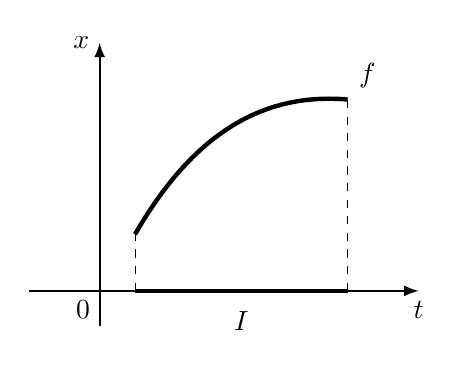
\begin{tikzpicture}[scale=0.9, >=latex]
    \draw[->, thick] (-1,0) -- (4.5,0) node[below] {$t$};
    \draw[->, thick] (0,-0.5) -- (0,3.5) node[left] {$x$};
    \node[below left] at (0,0) {$0$};

    \draw[ultra thick] (0.5, 0.8) to[out=60, in=175] (3.5, 2.7) node[above right] {$f$};

    \draw[dashed] (0.5, 0) -- (0.5, 0.8);
    \draw[dashed] (3.5, 0) -- (3.5, 2.7);

    \draw[ultra thick] (0.5, 0) -- (3.5, 0);
    \node[below=4pt] at (2,0) {$I$};
\end{tikzpicture}
\end{center}

O que é mais razoável esperar que ocorra: $f''(t) \le 0$ ou $f''(t) > 0$ em $I$? Por quê?
\linkresolucao{7.15.5}
\end{exercicio}

\begin{exercicio}[6]
\label{ex:7.15.6}
Seja $x = f(t)$, $t \ge 0$, tal que $f(0) = 1$ e $f(1) = 2$. Suponha, ainda, que $\deriv{x}{t} > 0$ para $t \ge 0$, $\dfrac{\diff^2x}{\diff t^2} < 0$ para $0 < t < 1$ e $\dfrac{\diff^2x}{\diff t^2} > 0$ para $t > 1$. Como você acha que deve ser o gráfico de $f$? Por quê?
\linkresolucao{7.15.6}
\end{exercicio}

\begin{exercicio}[7]
\label{ex:7.15.7}
Seja $f(t) = t^3 + 3t^2$.
\begin{enumerate}[label=\alph*)]
    \item Estude o sinal de $f'(t)$.
    \item Estude o sinal de $f''(t)$.
    \item Calcule $\lim\limits_{t \to +\infty} (t^3 + 3t^2)$ e $\lim\limits_{t \to -\infty} (t^3 + 3t^2)$.
    \item Utilizando as informações acima, esboce o gráfico de $f$.
\end{enumerate}
\linkresolucao{7.15.7}
\end{exercicio}

\begin{exercicio}[8]
\label{ex:7.15.8}
Seja $f(t) = \dfrac{t}{t^2 + 4}$.
\begin{enumerate}[label=\alph*)]
    \item Estude o sinal de $f'(t)$.
    \item Estude o sinal de $f''(t)$.
    \item Calcule $\lim\limits_{t \to +\infty} \dfrac{t}{t^2 + 4}$ e $\lim\limits_{t \to -\infty} \dfrac{t}{t^2 + 4}$.
    \item Utilizando as informações acima, esboce o gráfico de $f$.
\end{enumerate}
\linkresolucao{7.15.8}
\end{exercicio}

\begin{exercicio}[9]
\label{ex:7.15.9}
A posição de uma partícula que se desloca ao longo do eixo $x$ varia com o tempo segundo a equação $x = \dfrac{v_0}{k}(1 - e^{-kt})$, $t \ge 0$, em que $v_0$ e $k$ são constantes estritamente positivas.
\begin{enumerate}[label=\alph*)]
    \item Qual a velocidade no instante $t$?
    \item Com argumentos físicos, justifique a afirmação: ``a função é estritamente crescente.''
    \item Qual a aceleração no instante $t$?
    \item Com argumentos físicos, justifique a afirmação: ``o gráfico da função tem a concavidade voltada para baixo.''
    \item Calcule $\lim\limits_{t \to +\infty} \dfrac{v_0}{k}(1 - e^{-kt})$.
    \item Esboce o gráfico da função.
\end{enumerate}
\linkresolucao{7.15.9}
\end{exercicio}

\begin{exercicio}[10]
\label{ex:7.15.10}
A equação do movimento de uma partícula que se desloca ao longo do eixo $x$ é $x = e^{-t}\sen t$, $t \ge 0$.
\begin{enumerate}[label=\alph*)]
    \item Determine a velocidade e a aceleração no instante $t$.
    \item Calcule $\lim\limits_{t \to +\infty} e^{-t}\sen t$.
    \item Esboce o gráfico da função.
    \item Interprete tal movimento.
\end{enumerate}
\linkresolucao{7.15.10}
\end{exercicio}

\begin{exercicio}[11]
\label{ex:7.15.11}
Um ponto $P$ move-se sobre a parábola $y = 3x^2 - 2x$. Suponha que as coordenadas $x(t)$ e $y(t)$ de $P$ são deriváveis e que $\deriv{x}{t} \neq 0$. Pergunta-se: em que ponto da parábola a velocidade da ordenada $y$ de $P$ é o triplo da velocidade da abscissa $x$ de $P$?
\linkresolucao{7.15.11}
\end{exercicio}

\begin{exercicio}[12]
\label{ex:7.15.12}
Um ponto $P$ move-se ao longo do gráfico de $y = \dfrac{1}{x^2 + 1}$ de tal modo que a sua abscissa $x$ varia a uma velocidade constante de $5\text{ m/s}$. Qual a velocidade de $y$ no instante em que $x = 10\text{ m}$?
\linkresolucao{7.15.12}
\end{exercicio}

\begin{exercicio}[13]
\label{ex:7.15.13}
Um ponto desloca-se sobre a hipérbole $xy = 4$ de tal modo que a velocidade de $y$ é $\deriv{y}{t} = \beta$, $\beta$ constante. Mostre que a aceleração da abscissa $x$ é $\dfrac{\diff^2x}{\diff t^2} = \dfrac{\beta^2}{8}x^3$.
\linkresolucao{7.15.13}
\end{exercicio}

\begin{exercicio}[14]
\label{ex:7.15.14}
Seja um ponto move-se ao longo da elipse $x^2 + 4y^2 = 1$. A abscissa $x$ está variando a uma velocidade $\deriv{x}{t} = \sen 4t$. Mostre que:
\begin{enumerate}[label=\alph*)]
    \item $\deriv{y}{t} = -\dfrac{x\sen 4t}{4y}$
    \item $\dfrac{\diff^2y}{\diff t^2} = -\dfrac{\sen^2 4t + 16xy^2 \cos 4t}{16y^3}$
\end{enumerate}
\linkresolucao{7.15.14}
\end{exercicio}

\begin{exercicio}[15]
\label{ex:7.15.15}
Um ponto move-se sobre a semicircunferência $x^2 + y^2 = 5$, $y \ge 0$. Suponha $\deriv{x}{t} > 0$. Determine o ponto da curva em que a velocidade de $y$ seja o dobro da de $x$.
\linkresolucao{7.15.15}
\end{exercicio}

\begin{exercicio}[16]
\label{ex:7.15.16}
Uma escada de $8\text{ m}$ está encostada em uma parede. Se a extremidade inferior da escada for afastada do pé da parede a uma velocidade constante de $2\text{ m/s}$, com que velocidade a extremidade superior estará descendo no instante em que a inferior estiver a $3\text{ m}$ da parede?
\linkresolucao{7.15.16}
\end{exercicio}

\begin{exercicio}[17]
\label{ex:7.15.17}
Suponha que os comprimentos dos segmentos $AB$ e $OB$ sejam, respectivamente, $5\text{ cm}$ e $3\text{ cm}$. Suponha, ainda, que $\theta$ esteja variando a uma taxa constante de $\dfrac{1}{2}\text{ rad/s}$. Determine a velocidade de $A$, quando $\theta = \dfrac{\pi}{2}\text{ rad}$.
\begin{center}
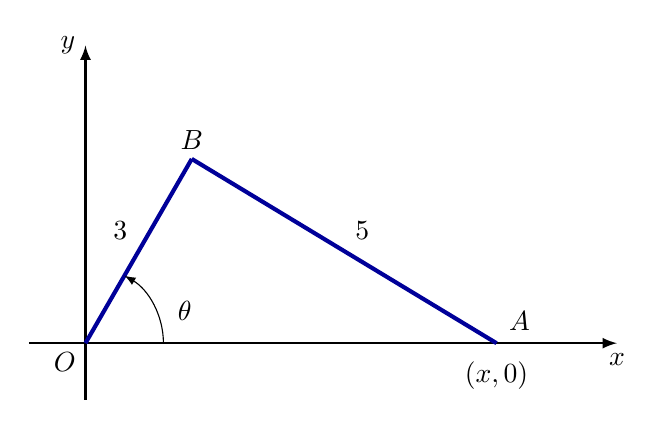
\begin{tikzpicture}[scale=0.9, >=latex]
    \draw[->, thick] (-0.8, 0) -- (7.5, 0) node[below] {$x$};
    \draw[->, thick] (0, -0.8) -- (0, 4.2) node[left] {$y$};
    \node[below left] at (0, 0) {$O$};
    
    \coordinate (O) at (0, 0);
    \coordinate (B) at (1.5, 2.6);
    \coordinate (A) at (5.8, 0);
    
    \draw[line width=1.5pt, blue!60!black] (O) -- (B) node[midway, above left, text=black] {$3$};
    \draw[line width=1.5pt, blue!60!black] (B) -- (A) node[midway, above right, text=black] {$5$};
    
    \node[above] at (B) {$B$};
    \node[above right=1pt] at (A) {$A$};
    \node[below=3pt] at (A) {$(x, 0)$};
    
    \draw[->] (1.1, 0) arc (0:60:1.1);
    \node at (1.4, 0.45) {$\theta$};
\end{tikzpicture}
\end{center}
\linkresolucao{7.15.17}
\end{exercicio}

\begin{exercicio}[18]
\label{ex:7.15.18}
Enche-se um reservatório, cuja forma é a de um cone circular reto, de água a uma taxa de $0{,}1\text{ m}^3\text{/s}$. O vértice está a $15\text{ m}$ do topo e o raio do topo é de $10\text{ m}$. Com que velocidade o nível $h$ da água está subindo no instante em que $h = 5\text{ m}$.

\begin{center}
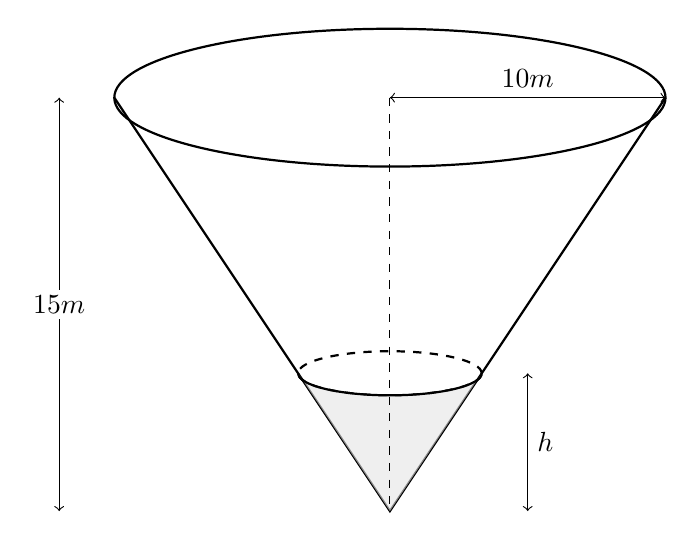
\begin{tikzpicture}[scale=0.35]
    \draw[thick] (0,15) ellipse (10 and 2.5);
    \draw[thick] (-10,15) -- (0,0) -- (10,15);
    \draw[thick, dashed] (0,5) ellipse (3.33 and 0.8);
    \fill[gray!20, opacity=0.6] (-3.33,5) -- (0,0) -- (3.33,5) arc (0:-180:3.33 and 0.8) -- cycle;
    \draw[thick] (-3.33,5) arc (-180:0:3.33 and 0.8);
    
    \draw[dashed] (0,15) -- (0,0);
    \draw[<->] (-12,0) -- (-12,15) node[midway, fill=white, inner sep=2pt] {$15\text{ m}$};
    \draw[<->] (5,0) -- (5,5) node[midway, right] {$h$};
    \draw[<->] (0,15) -- (10,15) node[midway, above] {$10\text{ m}$};
\end{tikzpicture}
\end{center}
\linkresolucao{7.15.18}
\end{exercicio}

\begin{exercicio}[19]
\label{ex:7.15.19}
O ponto $P = (x, y)$ está fixo à roda de raio $1\text{ m}$, que rola, sem escorregamento, sobre o eixo $x$. O ângulo $\theta$ está variando a uma taxa constante de $1\text{ rad/s}$. Expresse as velocidades da abscissa e da ordenada de $P$ em função de $\theta$.
\begin{center}
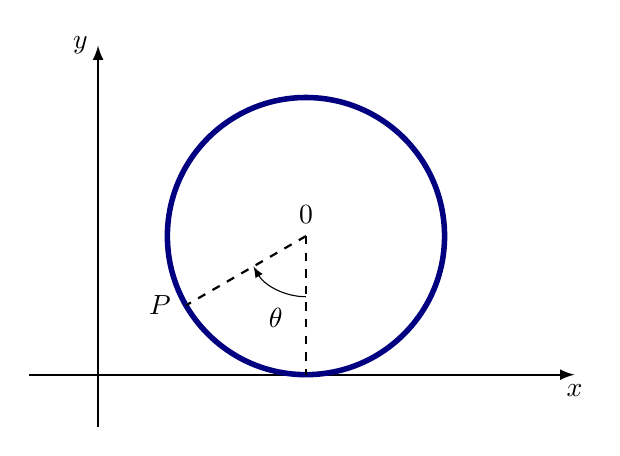
\begin{tikzpicture}[scale=1.1, >=latex]
    \draw[->, thick] (-0.8, 0) -- (5.5, 0) node[below] {$x$};
    \draw[->, thick] (0, -0.6) -- (0, 3.8) node[left] {$y$};
    
    \coordinate (C) at (2.4, 1.6);
    \draw[line width=2pt, blue!50!black] (C) circle (1.6);
    \node[above=1pt] at (C) {$0$};
    
    \coordinate (T) at (2.4, 0);
    \draw[dashed, thick] (C) -- (T);
    
    \path (C) ++(210:1.6) coordinate (P);
    \draw[dashed, thick] (C) -- (P);
    \node[left=2pt] at (P) {$P$};
    
    \draw[->] (2.4, 0.9) arc (-90:-150:0.7);
    \node at (2.05, 0.65) {$\theta$};
\end{tikzpicture}
\end{center}
\linkresolucao{7.15.19}
\end{exercicio}

\begin{exercicio}[20]
\label{ex:7.15.20}
Um ponto $P$ move-se sobre a parábola $y^2 = x$, $x > 0$ e $y > 0$. A abscissa $x$ está variando com uma aceleração que, em cada instante, é o dobro do quadrado da velocidade da ordenada $y$. Mostre que a ordenada está variando com aceleração nula.
\linkresolucao{7.15.20}
\end{exercicio}

\begin{exercicio}[21]
\label{ex:7.15.21}
Dois pontos $P$ e $Q$ deslocam-se, respectivamente, nos eixos $x$ e $y$ de modo que a soma das distâncias de $P$ a $R$ e de $R$ a $Q$ mantém-se constante e igual a $e$ durante o movimento, em que $R = (0, h)$ é um ponto fixo. (Veja a figura a seguir.)

\begin{center}
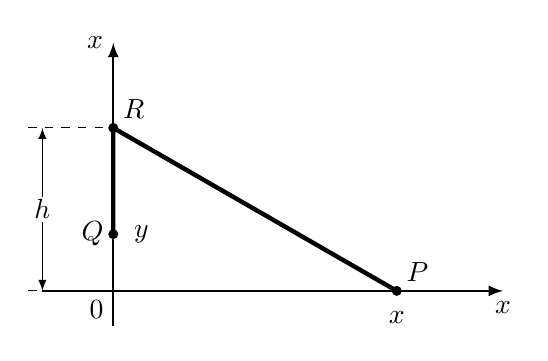
\begin{tikzpicture}[scale=0.9, >=latex]
    \draw[->, thick] (-1,0) -- (5.5,0) node[below] {$x$};
    \draw[->, thick] (0,-0.5) -- (0,3.5) node[left] {$x$};
    \node[below left] at (0,0) {$0$};
    
    \coordinate (R) at (0,2.3);
    \coordinate (Q) at (0,0.8);
    \coordinate (P) at (4,0);
    
    \draw[ultra thick] (Q) -- (R) -- (P);
    
    \fill (R) circle (2pt) node[above right] {$R$};
    \fill (Q) circle (2pt) node[left] {$Q$} node[right=4pt] {$y$};
    \fill (P) circle (2pt) node[above right] {$P$} node[below=4pt] {$x$};
    
    \draw[dashed] (-1.2, 2.3) -- (0, 2.3);
    \draw[dashed] (-1.2, 0) -- (0, 0);
    \draw[<->] (-1, 0) -- (-1, 2.3) node[midway, fill=white, inner sep=1pt] {$h$};
\end{tikzpicture}
\end{center}

Relacione a velocidade $\deriv{y}{t}$ de $Q$ com a velocidade $\deriv{x}{t}$ de $P$.
\linkresolucao{7.15.21}
\end{exercicio}

\clearpage

% ------------------------------------------------------------------------------
% 7.16. PROBLEMAS RETA TANGENTE E NORMAL AO GRÁFICO DE UMA FUNÇÃO
% ------------------------------------------------------------------------------
\subsection{Problemas Reta Tangente e Normal ao Gráfico de uma Função}

\begin{exercicio}[1]
\label{ex:7.16.1}
Determine as equações das retas tangente e normal ao gráfico da função dada, no ponto dado:
\begin{enumerate}[label=\alph*)]
    \item $f(x) = x^2 - 3x$, no ponto de abscissa 0
    \item $f(x) = \sqrt[3]{x}$, no ponto de abscissa 8
    \item $g(x) = \dfrac{1}{x^2}$, no ponto de abscissa 1
    \item $g(x) = x + \dfrac{1}{x}$, no ponto de abscissa 1
\end{enumerate}
\linkresolucao{7.16.1}
\end{exercicio}

\begin{exercicio}[2]
\label{ex:7.16.2}
Seja $f(x) = x^2$. Determine a equação da reta que é tangente ao gráfico de $f$ e paralela à reta $y = \dfrac{1}{2}x + 3$.
\linkresolucao{7.16.2}
\end{exercicio}

\begin{exercicio}[3]
\label{ex:7.16.3}
Sabe-se que $r$ é uma reta tangente ao gráfico de $f(x) = x^3 + 3x$ e paralela à reta $y = 6x - 1$. Determine $r$.
\linkresolucao{7.16.3}
\end{exercicio}

\begin{exercicio}[4]
\label{ex:7.16.4}
Determine a equação da reta que é perpendicular à reta $2y + x = 3$ e tangente ao gráfico de $f(x) = x^2 - 3x$.
\linkresolucao{7.16.4}
\end{exercicio}

\begin{exercicio}[5]
\label{ex:7.16.5}
Sabe-se que $r$ é uma reta perpendicular à reta $3x + y = 3$ e tangente ao gráfico de $f(x) = x^3$. Determine $r$.
\linkresolucao{7.16.5}
\end{exercicio}

\begin{exercicio}[6]
\label{ex:7.16.6}
Seja a reta $s$ passa pelo ponto $(3, 0)$ e é normal ao gráfico de $f(x) = x^2$ no ponto $(a, b)$:
\begin{enumerate}[label=\alph*)]
    \item Determine $(a, b)$.
    \item Determine a equação de $s$.
\end{enumerate}
\linkresolucao{7.16.6}
\end{exercicio}

\begin{exercicio}[7]
\label{ex:7.16.7}
Sabe-se que $r$ é uma reta que passa pela origem e que é tangente ao gráfico de $f(x) = x^3 + 2x^2 - 3x$. Determine $r$.
\linkresolucao{7.16.7}
\end{exercicio}

\begin{exercicio}[8]
\label{ex:7.16.8}
Determine todos os pontos $(a, b)$ sobre a curva $y = x^4 + 2x^3 - 2x^2 + 8x + 12$ tais que a reta tangente em $(a, b)$ seja paralela à reta $8x - y + \pi = 0$.
\linkresolucao{7.16.8}
\end{exercicio}

\begin{exercicio}[9]
\label{ex:7.16.9}
Determine todos os pontos $(a, b)$ sobre o gráfico da função dada por $y = 4x^3 + x^2 - 4x - 1$ tais que a reta tangente em $(a, b)$ seja paralela ao eixo $x$.
\linkresolucao{7.16.9}
\end{exercicio}

\begin{exercicio}[10]
\label{ex:7.16.10}
Sabe-se que $r$ é uma reta que passa pelo ponto $(0, 2)$ e que é tangente ao gráfico de $f(x) = x^3$. Determine $r$.
\linkresolucao{7.16.10}
\end{exercicio}

\begin{exercicio}[11]
\label{ex:7.16.11}
Determine a equação de uma reta, não vertical, que passa pelo ponto $\left(0, \dfrac{4}{3}\right)$ e que seja normal ao gráfico de $y = x^3$.
\linkresolucao{7.16.11}
\end{exercicio}

\begin{exercicio}[12]
\label{ex:7.16.12}
Determine todos os pontos $(a, b)$ de $\R^2$ tais que por $(a, b)$ passem duas retas tangentes ao gráfico de $f(x) = x^2$.
\linkresolucao{7.16.12}
\end{exercicio}

\begin{exercicio}[13]
\label{ex:7.16.13}
Sejam $A$ e $B$ os pontos em que o gráfico de $f(x) = x^2 - \alpha x$, $\alpha$ real, intercepta o eixo $x$. Determine $\alpha$ para que as retas tangentes ao gráfico de $f$, em $A$ e em $B$, sejam perpendiculares.
\linkresolucao{7.16.13}
\end{exercicio}

\begin{exercicio}[14]
\label{ex:7.16.14}
Determine $\beta$ para que $y = \beta x - 2$ seja tangente ao gráfico de $f(x) = x^3 - 4x$.
\linkresolucao{7.16.14}
\end{exercicio}

\begin{exercicio}[15]
\label{ex:7.16.15}
Sabe-se que $r$ é uma reta tangente aos gráficos de $f(x) = -x^2$ e de $g(x) = \dfrac{1}{2} + x^2$. Determine $r$.
\linkresolucao{7.16.15}
\end{exercicio}

\clearpage

% ------------------------------------------------------------------------------
% 7.17. EXERCÍCIOS DO CAPÍTULO
% ------------------------------------------------------------------------------
\subsection{Exercícios do Capítulo}

\begin{exercicio}[1]
\label{ex:7.17.1}
Calcule, pela definição, a derivada da função dada, no ponto dado:
\begin{enumerate}[label=\alph*)]
    \item $f(x) = \dfrac{1}{x + 1}$ em $p = 2$
    \item $g(x) = \sqrt{2x + 1}$ em $p = 0$
    \item $y = \sen \pi x$ em $p = 1$
    \item $f(x) = e^{x^2}$ em $p = 0$
    \item $g(x) = \begin{cases} x^{3/2} \sen \dfrac{1}{x^2} & \text{se } x \neq 0 \\ 0 & \text{se } x = 0 \end{cases}$ em $p = 0$
    \item $g(x) = \sqrt{x^2 + x}$ em $p = 1$
    \item $y = \cos x^2$ em $p = 0$
    \item $y = \sqrt{1 + \sqrt{x}}$ em $p = 1$
    \item $y = x^x$ em $p = 1$ (Sugestão: Veja Exemplo 3-6.3.)
\end{enumerate}
\linkresolucao{7.17.1}
\end{exercicio}

\begin{exercicio}[2]
\label{ex:7.17.2}
Calcule a derivada:
\begin{enumerate}[label=\alph*)]
    \item $y = \sqrt{1 + \sqrt{x}}$
    \item $y = \ln(3x + \sqrt{1 + 9x^2})$
    \item $y = x\,5^{x^2}$
    \item $y = (2 + \sen x)^x$
    \item $y = \ln\sqrt{\dfrac{1 + \sen x}{1 - \sen x}}$
    \item $x = e^{t^2}\sen 3t$
    \item $s = t\ln\dfrac{t^2 - 1}{t^2 + 1}$
    \item $y = \dfrac{x^2 + 1}{\sqrt{x + 1}}$
    \item $y = \dfrac{t^3}{(t^2 + 1)^2}$
    \item $f(x) = \dfrac{x\tg 3x}{x^2 + 4}$
    \item $y = \ln\dfrac{1 + \tg\dfrac{x}{2}}{1 - \tg\dfrac{x}{2}}$
    \item $g(x) = \dfrac{e^{\sec\sqrt{x}}}{x}$
    \item $y = e^{x^x}$
    \item $y = \dfrac{1}{2}\tg^2 x + \ln\cos x$
    \item $y = \ln\!\left[\dfrac{\sqrt{1 - x} + \sqrt{1 + x}}{\sqrt{1 - x} - \sqrt{1 + x}}\right] - \dfrac{\sqrt{1 - x^2}}{x}$
    \item $y = \dfrac{2(4 + 3\sqrt[3]{x})(2 - \sqrt[3]{x})^2}{5}$
    \item $s = \dfrac{2^{3t} - 2^{-3t}}{2^{3t} + 2^{-3t}}$
    \item $f(x) = \ln\dfrac{\cos\sqrt{x}}{1 + \sen\sqrt{x}}$
    \item $y = e^{-3x}(\cos 3x - \sen 3x)$
    \item $y = \dfrac{1}{2}\cotg^2 5x + \ln\sen 5x$
\end{enumerate}
\linkresolucao{7.17.2}
\end{exercicio}

\begin{exercicio}[3]
\label{ex:7.17.3}
Expresse $\deriv{y}{x}$ em termos de $x$ e de $y$, em que $y = y(x)$ é uma função derivável, dada implicitamente pela equação dada:
\begin{enumerate}[label=\alph*)]
    \item $y^3 + \sen xy = 1$
    \item $e^y + xy = x$
    \item $y^x + x = y^2$
    \item $x\cos y + y\cos x = 2$
\end{enumerate}
\linkresolucao{7.17.3}
\end{exercicio}

\begin{exercicio}[4]
\label{ex:7.17.4}
Seja $y = f(x)$ definida e derivável num intervalo contendo 1 e suponha que $f$ seja dada implicitamente pela equação $y^3 + x^2 y = 130$. Determine as equações das retas tangente e normal ao gráfico de $f$, no ponto de abscissa 1.
\linkresolucao{7.17.4}
\end{exercicio}

\begin{exercicio}[5]
\label{ex:7.17.5}
Determine uma reta que seja paralela a $x + y = 1$ e que seja tangente à curva $x^2 + xy + y^2 = 3$.
\linkresolucao{7.17.5}
\end{exercicio}

\begin{exercicio}[6]
\label{ex:7.17.6}
Determine uma reta que seja tangente à elipse $x^2 + 2y^2 = 9$ e que intercepta o eixo $y$ no ponto de ordenada $\dfrac{9}{4}$.
\linkresolucao{7.17.6}
\end{exercicio}

\begin{exercicio}[7]
\label{ex:7.17.7}
Mostre que a reta $\dfrac{x}{x_0} + \dfrac{y}{y_0} = 2$ é tangente à curva $\left(\dfrac{x}{x_0}\right)^{\!3} + \left(\dfrac{y}{y_0}\right)^{\!3} = 2$ no ponto $(x_0, y_0)$.
\linkresolucao{7.17.7}
\end{exercicio}

\begin{exercicio}[8]
\label{ex:7.17.8}
Determine uma reta paralela a $x + y = 1$ e tangente à curva $y^3 + xy + x^3 = 0$ em um ponto $(x_0, y_0)$, com $x_0 < 0$ e $y_0 < 0$.
\linkresolucao{7.17.8}
\end{exercicio}

\begin{exercicio}[9]
\label{ex:7.17.9}
Os lados $x$ e $y$ de um retângulo estão variando a taxas constantes de $0{,}2\text{ m/s}$ e $0{,}1\text{ m/s}$, respectively. A que taxa estará variando a área do retângulo no instante em que $x = 1\text{ m}$ e $y = 2\text{ m}$?
\linkresolucao{7.17.9}
\end{exercicio}

\begin{exercicio}[10]
\label{ex:7.17.10}
A altura $h$ e o raio $r$ da base de um cone circular reto estão variando a taxas constantes de $0{,}1\text{ m/s}$ e $0{,}3\text{ m/s}$, respectivamente. A que taxa estará variando o volume do cone no instante em que $h = 0{,}5\text{ m}$ e $r = 0{,}2\text{ m}$?
\linkresolucao{7.17.10}
\end{exercicio}

\begin{exercicio}[11]
\label{ex:7.17.11}
O volume $V$ e o raio $r$ da base de um cone circular reto estão variando a taxas constantes de $0{,}1\,\pi\text{ m}^3\text{/s}$ e $0{,}2\text{ m/s}$, respectivamente. Expresse $\deriv{h}{t}$ em termos de $r$ e $h$, em que $h$ é a altura do cone.
\linkresolucao{7.17.11}
\end{exercicio}

\begin{exercicio}[12]
\label{ex:7.17.12}
Num determinado instante, as arestas de um paralelepípedo medem $a$, $b$, $c$ (m) e, neste instante, estão variando com velocidades $v_a$, $v_b$ e $v_c$ (m/s), respectivamente. Mostre que neste instante o volume do paralelepípedo estará variando a uma taxa de $v_a bc + a v_b c + ab v_c$ ($\text{m}^3\text{/s}$).
\linkresolucao{7.17.12}
\end{exercicio}

\begin{exercicio}[13]
\label{ex:7.17.13}
O raio $r$ e a altura $h$ de um cilindro circular reto estão variando de modo a manter constante o volume $V$. Num determinado instante $h = 3\text{ cm}$ e $r = 1\text{ cm}$ e, neste instante, a altura está variando a uma taxa de $0{,}2\text{ cm/s}$. A que taxa estará variando o raio neste instante?
\linkresolucao{7.17.13}
\end{exercicio}

\begin{exercicio}[14]
\label{ex:7.17.14}
Uma piscina tem $10\text{ m}$ de largura, $20\text{ m}$ de comprimento, $1\text{ m}$ de profundidade nas extremidades e $3\text{ m}$ no meio, de modo que o fundo seja formado por dois planos inclinados. Despeja-se água na piscina a uma taxa de $0{,}3\text{ m}^3\text{/min}$. Seja $h$ a altura da água em relação à parte mais profunda. Com que velocidade $h$ estará variando no instante em que $h = 1\text{ m}$?

\begin{center}
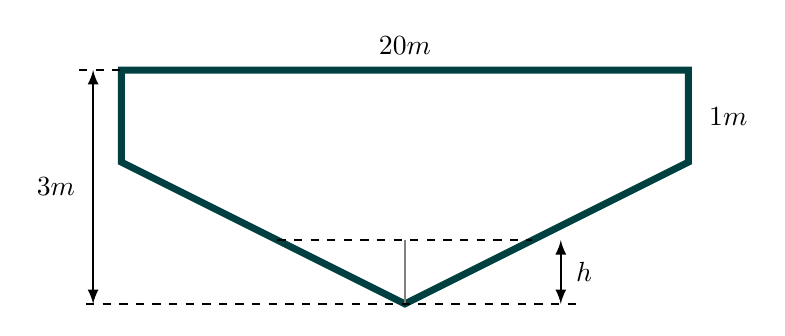
\begin{tikzpicture}[scale=0.9, >=latex]
    \draw[line width=2.5pt, teal!50!black] 
        (-4, 2) -- (4, 2) -- (4, 0.7) -- (0, -1.3) -- (-4, 0.7) -- cycle;

    \draw[dashed, thick] (-1.8, -0.4) -- (1.8, -0.4);
    \draw[gray, thick] (0, -1.3) -- (0, -0.4);
    \draw[dashed, thick] (-4.5, -1.3) -- (2.5, -1.3);

    \node[above=2pt] at (0, 2) {$20\text{ m}$};
    \node[right=4pt] at (4, 1.35) {$1\text{ m}$};

    \draw[dashed] (-4.6, 2) -- (-4, 2);
    \draw[<->, thick] (-4.4, -1.3) -- (-4.4, 2);
    \node[left=3pt] at (-4.4, 0.35) {$3\text{ m}$};

    \draw[<->, thick] (2.2, -1.3) -- (2.2, -0.4);
    \node[right=2pt] at (2.2, -0.85) {$h$};
\end{tikzpicture}
\end{center}
\linkresolucao{7.17.14}
\end{exercicio}

\begin{exercicio}[15]
\label{ex:7.17.15}
Num determinado instante $\theta = \dfrac{\pi}{3}$ e está variando, neste instante, a uma taxa de $0{,}01\text{ rad/s}$ (veja figura). A que taxa estará variando o ângulo $\alpha$ neste instante?

\begin{center}
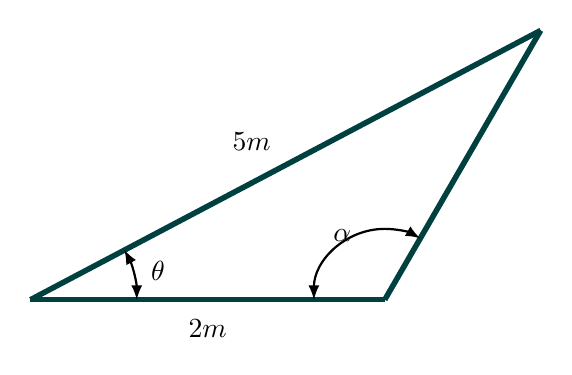
\begin{tikzpicture}[scale=0.9, >=latex]
    \coordinate (O) at (0, 0);
    \coordinate (A) at (5, 0);
    \coordinate (B) at (7.2, 3.8);

    \draw[line width=2pt, teal!50!black] (O) -- (A) node[midway, below=3pt, text=black] {$2\text{ m}$};
    \draw[line width=2pt, teal!50!black] (O) -- (B) node[midway, above left=1pt, text=black] {$5\text{ m}$};
    \draw[line width=2pt, teal!50!black] (A) -- (B);

    \draw[<->, thick] (1.5, 0) arc (0:28:1.5);
    \node at (1.8, 0.4) {$\theta$};

    \draw[<->, thick] (4, 0) arc (180:60:1);
    \node at (4.4, 0.9) {$\alpha$};
\end{tikzpicture}
\end{center}
\linkresolucao{7.17.15}
\end{exercicio}

\begin{exercicio}[16]
\label{ex:7.17.16}
Com relação ao exercício anterior, supondo $\dfrac{\pi}{2} < \alpha < \pi$, expresse $\deriv{\alpha}{t}$ em termos de $\theta$ e $\deriv{\theta}{t}$.
\linkresolucao{7.17.16}
\end{exercicio}

\begin{exercicio}[17]
\label{ex:7.17.17}
Considere as funções dadas por $y = ax^2$ e $y = -x^2 + 1$. Determine $a$ para que os gráficos se interceptem ortogonalmente. (Os gráficos se interceptam ortogonalmente em $(x_0, y_0)$ se as retas tangentes aos gráficos, neste ponto, forem perpendiculares.)
\linkresolucao{7.17.17}
\end{exercicio}

\begin{exercicio}[18]
\label{ex:7.17.18}
Determine $a$ para que as circunferências $x^2 + y^2 = 1$ e $(x - a)^2 + y^2 = 1$ se interceptem ortogonalmente.
\linkresolucao{7.17.18}
\end{exercicio}

\begin{exercicio}[19]
\label{ex:7.17.19}
Mostre que, para todo $a$, as curvas $y = ax^2$ e $x^2 + 2y^2 = 1$ se interceptam ortogonalmente.
\linkresolucao{7.17.19}
\end{exercicio}

\begin{exercicio}[20]
\label{ex:7.17.20}
Seja $f\colon \R \to \R$ derivável e considere a função dada por $y = x^2 f(x^2 + 1)$.
\begin{enumerate}[label=\alph*)]
    \item Verifique que $\deriv{y}{x} = 2x f(x^2 + 1) + 2x^3 f'(x^2 + 1)$
    \item Expresse $\left.\deriv{y}{x}\right|_{x = 1}$ em termos de $f(2)$ e $f'(2)$
\end{enumerate}
\linkresolucao{7.17.20}
\end{exercicio}

\begin{exercicio}[21]
\label{ex:7.17.21}
Seja $\phi$ a função dada por $\phi(x) = x^2 + 1$. Calcule:
\begin{enumerate}[label=\alph*)]
    \item $\phi'(\phi(x))$
    \item $(\phi(\phi(x)))'$
\end{enumerate}
\linkresolucao{7.17.21}
\end{exercicio}

\begin{exercicio}[22]
\label{ex:7.17.22}
Calcule $\phi'(\phi(x))$ sendo $\phi$ dada por:
\begin{enumerate}[label=\alph*)]
    \item $\phi(x) = \sen x$
    \item $\phi(x) = \dfrac{1}{x}$
    \item $\phi(x) = \ln(x^2 + 1)$
    \item $\phi(x) = e^{x^2}$
\end{enumerate}
\linkresolucao{7.17.22}
\end{exercicio}

\begin{exercicio}[23]
\label{ex:7.17.23}
Para cada $\phi$ do exercício anterior, calcule $(\phi(\phi(x)))'$.
\linkresolucao{7.17.23}
\end{exercicio}

\begin{exercicio}[24]
\label{ex:7.17.24}
Dê exemplos de funções $\phi$ que satisfazem a condição $\phi'(\phi(x)) = (\phi(\phi(x)))'$, para todo $x$ no domínio de $\phi$.
\linkresolucao{7.17.24}
\end{exercicio}

\begin{exercicio}[25]
\label{ex:7.17.25}
Considere uma partícula que se desloca sobre o eixo $x$ com função de posição $x = \cos 3t$.
\begin{enumerate}[label=\alph*)]
    \item Verifique que a aceleração é proporcional à posição.
    \item Calcule a aceleração no instante em que a partícula se encontra na posição $x = -\dfrac{1}{2}$.
\end{enumerate}
\linkresolucao{7.17.25}
\end{exercicio}

\begin{exercicio}[26]
\label{ex:7.17.26}
Considere uma partícula que se desloca sobre o eixo $x$ com função de posição $x = \dfrac{1}{2t + 1}$.
\begin{enumerate}[label=\alph*)]
    \item Verifique que a aceleração é proporcional ao cubo da posição.
    \item Qual a aceleração no instante em que a partícula se encontra na posição $x = \sqrt[3]{7}$?
\end{enumerate}
\linkresolucao{7.17.26}
\end{exercicio}

\begin{exercicio}[27]
\label{ex:7.17.27}
Seja $f\colon \R \to \R$ derivável até a 2\textsuperscript{a} ordem e seja $h$ dada por $h(t) = f'(\cos 3t)$.
\begin{enumerate}[label=\alph*)]
    \item Expresse $h''(t)$ em termos de $t$, $f'(\cos 3t)$ e de $f''(\cos 3t)$.
    \item Calcule $h''\!\left(\dfrac{\pi}{9}\right)$ admitindo que $f'\!\left(\dfrac{1}{2}\right) = 4$ e $f''\!\left(\dfrac{1}{2}\right) = 3$.
\end{enumerate}
\linkresolucao{7.17.27}
\end{exercicio}

\begin{exercicio}[28]
\label{ex:7.17.28}
Suponha que $y = y(t)$ seja uma função derivável tal que para todo $t$ no seu domínio $\deriv{y}{t} = ty^2$.
\begin{enumerate}[label=\alph*)]
    \item Expresse $\dfrac{\diff^2 y}{\diff t^2}$ em termos de $t$ e de $y$.
    \item Calcule $\left.\dfrac{\diff^2 y}{\diff t^2}\right|_{t = 1}$ supondo que $y(1) = 1$.
\end{enumerate}
\linkresolucao{7.17.28}
\end{exercicio}

\begin{exercicio}[29]
\label{ex:7.17.29}
Seja $y = y(x)$ definida e derivável num intervalo $I$ e tal que, para todo $x$ em $I$, $\deriv{y}{x} = x + \sen y$.
\begin{enumerate}[label=\alph*)]
    \item Expresse $\dfrac{\diff^3 y}{\diff x^3}$ em termos de $x$ e de $y$.
    \item Calcule $\left.\dfrac{\diff^3 y}{\diff x^3}\right|_{x = 0}$ admitindo que $y(0) = \dfrac{\pi}{4}$.
\end{enumerate}
\linkresolucao{7.17.29}
\end{exercicio}

\begin{exercicio}[30]
\label{ex:7.17.30}
Seja $f\colon \R \to \R$ derivável até a 2\textsuperscript{a} ordem e tal que, para todo $x$:
\[
f''(x) + 4f(x) = 0.
\]
Mostre que, para todo $x$:
\[
\frac{\diff}{\diff x}[f'(x)\sen 2x - 2\cos 2x\,f(x)] = 0.
\]
\linkresolucao{7.17.30}
\end{exercicio}

\begin{exercicio}[31]
\label{ex:7.17.31}
Sejam $f\colon \R \to \R$ derivável até a 2\textsuperscript{a} ordem e $h$ dada por $h(x) = f(f(x))$. Verifique que, para todo $x$, $h''(x) = f''(f(x))(f'(x))^2 + f'(f(x))f''(x)$.
\linkresolucao{7.17.31}
\end{exercicio}

\begin{exercicio}[32]
\label{ex:7.17.32}
Considere o polinômio
\[
P(x) = A_0 + A_1 (x - x_0) + A_2 (x - x_0)^2 + A_3 (x - x_0)^3
\]
em que $A_0$, $A_1$, $A_2$, $A_3$ e $x_0$ são números reais fixos. Mostre que:
\[
P(x) = P(x_0) + P'(x_0)(x - x_0) + \dfrac{P''(x_0)}{2!}(x - x_0)^2 + \dfrac{P'''(x_0)}{3!}(x - x_0)^3.
\]
\linkresolucao{7.17.32}
\end{exercicio}

\begin{exercicio}[33]
\label{ex:7.17.33}
Considere o polinômio $P(x) = a_0 + a_1 x + a_2 x^2 + a_3 x^3$ em que $a_0$, $a_1$, $a_2$ e $a_3$ são reais fixos. Seja $x_0$ um real dado.
\begin{enumerate}[label=\alph*)]
    \item Mostre que existem constantes $A_0$, $A_1$, $A_2$ e $A_3$ tais que
    \[
    P(x) = A_0 + A_1 (x - x_0) + A_2 (x - x_0)^2 + A_3 (x - x_0)^3.
    \]
    (Sugestão: Faça $x = (x - x_0) + x_0$.)
    \item Conclua que
    \[
    P(x) = P(x_0) + P'(x_0)(x - x_0) + \dfrac{P''(x_0)}{2!}(x - x_0)^2 + \dfrac{P'''(x_0)}{3!}(x - x_0)^3.
    \]
\end{enumerate}
\linkresolucao{7.17.33}
\end{exercicio}

\begin{exercicio}[34]
\label{ex:7.17.34}
Determine o desenvolvimento de Taylor de $P(x) = x^3 + 2x + 3$, em potências de $(x - 1)$.
\linkresolucao{7.17.34}
\end{exercicio}

\begin{exercicio}[35]
\label{ex:7.17.35}
Generalize o resultado do Exercício 33.
\linkresolucao{7.17.35}
\end{exercicio}

\begin{exercicio}[36]
\label{ex:7.17.36}
Determine o desenvolvimento de Taylor de $P(x) = x^4 - 3x^2 + x + 1$ em potências de:
\begin{enumerate}[label=\alph*)]
    \item $x - 2$
    \item $x + 1$
\end{enumerate}
\linkresolucao{7.17.36}
\end{exercicio}

\begin{exercicio}[37]
\label{ex:7.17.37}
Sejam $P(x)$ e $Q(x)$ polinômios tais que $P(x_0) = 0$, $Q(x_0) = 0$ e $Q'(x_0) \neq 0$. Mostre que:
\[
\lim_{x \to x_0} \dfrac{P(x)}{Q(x)} = \dfrac{P'(x_0)}{Q'(x_0)}.
\]
(Sugestão: Desenvolva $P(x)$ e $Q(x)$ em potências de $x - x_0$ e simplifique.)
\linkresolucao{7.17.37}
\end{exercicio}

\begin{exercicio}[38]
\label{ex:7.17.38}
Sejam $P(x)$ e $Q(x)$ polinômios tais que $P(x_0) = P'(x_0) = 0$, $Q(x_0) = Q'(x_0) = 0$ e $Q''(x_0) \neq 0$. Mostre que $\lim\limits_{x \to x_0} \dfrac{P(x)}{Q(x)} = \dfrac{P''(x_0)}{Q''(x_0)}$. Generalize.
\linkresolucao{7.17.38}
\end{exercicio}

\begin{exercicio}[39]
\label{ex:7.17.39}
Utilizando os Exercícios 37 e 38, calcule:
\begin{enumerate}[label=\alph*)]
    \item $\lim\limits_{x \to 1} \dfrac{x^{100} + x - 2}{x^{99} - x}$
    \item $\lim\limits_{x \to 1} \dfrac{x^3 - x^2 - x + 1}{x^{10} - 9x^2 + 8x}$
    \item $\lim\limits_{x \to -1} \dfrac{x^5 + 3x + 4}{x^{20} + 3x + 2}$
    \item $\lim\limits_{x \to 1} \dfrac{x^4 - 2x^3 + 2x - 1}{x^8 - 6x^6 + 8x^5 - 3x^4}$
\end{enumerate}
\linkresolucao{7.17.39}
\end{exercicio}

\begin{exercicio}[40]
\label{ex:7.17.40}
Sejam $f$ e $g$ deriváveis em $p$ e tais que $f(p) = g(p) = 0$. Supondo $g'(p) \neq 0$, mostre que:
\[
\lim_{x \to p} \dfrac{f(x)}{g(x)} = \dfrac{f'(p)}{g'(p)}.
\]
\linkresolucao{7.17.40}
\end{exercicio}

\begin{exercicio}[41]
\label{ex:7.17.41}
Utilizando o Exercício 40, calcule:
\begin{enumerate}[label=\alph*)]
    \item $\lim\limits_{x \to 0} \dfrac{\ln(x + 1)}{x^2 + \sen x}$
    \item $\lim\limits_{x \to \frac{\pi}{2}} \dfrac{e^{2x - \pi} - 1}{2\sen x + \sen 6x - 2}$
    \item $\lim\limits_{x \to -1} \dfrac{\sqrt[3]{x} + 1}{\sen\pi x^2}$
    \item $\lim\limits_{x \to 0} \dfrac{x + \sqrt[3]{x^2} + \sen 3x}{\ln(x^2 + x + 1)}$
    \item $\lim\limits_{x \to 0} \dfrac{e^{-x^2} + x - 1}{e^{4x} + x^5 - 1}$
    \item $\lim\limits_{x \to 1} \dfrac{\sen(\sen\pi x)}{2 - \sqrt{x} - \sqrt[3]{x^2}}$
\end{enumerate}
\linkresolucao{7.17.41}
\end{exercicio}

\begin{exercicio}[42]
\label{ex:7.17.42}
Seja $f$ definida em $\R$ e derivável em $p$. Suponha $f'(p) > 0$. Prove que existe $r > 0$ tal que
\[
f(x) > f(p) \quad \text{em } {]p, p + r[}
\]
e
\[
f(x) < f(p) \quad \text{em } {]p - r, p[}.
\]
(Sugestão: Lembre-se da definição de derivada e utilize a conservação do sinal.)
\linkresolucao{7.17.42}
\end{exercicio}

\begin{exercicio}[43]
\label{ex:7.17.43}
Seja $f$ definida e derivável em $\R$ e sejam $a$ e $b$ raízes consecutivas de $f$. Mostre que:
\[
f'(a) \cdot f'(b) \le 0.
\]
\linkresolucao{7.17.43}
\end{exercicio}

\begin{exercicio}[44]
\label{ex:7.17.44}
Suponha $f$ derivável no intervalo $I$. Prove que se $f$ for estritamente crescente em $I$, então $f'(x) \ge 0$ em $I$.
\linkresolucao{7.17.44}
\end{exercicio}

\begin{exercicio}[45]
\label{ex:7.17.45}
Suponha $f$ derivável em $[a, b]$ e tal que $f'(a) \cdot f'(b) < 0$. Prove que existe $p$ em ${]a, b[}$ tal que $f(x) \le f(p)$ para todo $x$ em $[a, b]$ ou $f(x) \ge f(p)$ para todo $x$ em $[a, b]$. Interprete geometricamente.
\linkresolucao{7.17.45}
\end{exercicio}

\begin{exercicio}[46]
\label{ex:7.17.46}
Suponha $f$ derivável em $[a, b]$ tal que $f'(a) \cdot f'(b) > 0$ e $f(a) = f(b)$. Prove que existem $x_1, x_2 \in {]a, b[}$ tais que, para todo $x \in [a, b]$, $f(x_1) \le f(x) \le f(x_2)$. Interprete geometricamente.
\linkresolucao{7.17.46}
\end{exercicio}

\begin{exercicio}[47]
\label{ex:7.17.47}
Seja $f\colon \R \to \R$ uma função tal que quaisquer que sejam $x$ e $t$:
\[
|f(x) - f(t)| \le |x - t|^2.
\]
Calcule $f'(x)$.
\linkresolucao{7.17.47}
\end{exercicio}

\begin{exercicio}[48]
\label{ex:7.17.48}
Sejam $f$ e $g$ definidas em $\R$, com $g$ contínua em 0, e tais que, para todo $x$, $f(x) = xg(x)$. Mostre que $f$ é derivável em 0.
\linkresolucao{7.17.48}
\end{exercicio}

\begin{exercicio}[49]
\label{ex:7.17.49}
Suponha $f$ definida em $\R$, derivável em 0 e $f(0) = 0$. Prove que existe $g$ definida em $\R$, contínua em 0, tal que $f(x) = xg(x)$ para todo $x$.
\linkresolucao{7.17.49}
\end{exercicio}


% ==============================================================================
% PARTE 2: RESOLUÇÕES DO CAPÍTULO
% ==============================================================================
\clearpage
\section*{Resoluções do Capítulo 7}
\addcontentsline{toc}{section}{Resoluções do Capítulo 7}

% ==============================================================================
% 7.1. INTRODUÇÃO
% ==============================================================================
\subsection*{7.1. Introdução}
\textit{Esta subseção não possui exercícios.}

% ==============================================================================
% 7.2. DERIVADA DE UMA FUNÇÃO
% ==============================================================================
\subsection*{7.2. Derivada de uma função}

\vspace{0.6cm}
\noindent\textbf{Resolução do Exercício 1.}
\label{res:7.2.1}
\linkenunciado{7.2.1}

\begin{enumerate}[label=\alph*)]

    \item $f'(1)$
    \setcounter{equation}{0}

    Pela definição formal de derivada no ponto $p = 1$, temos:
    \begin{equation}
        f'(1) = \lim_{x \to 1} \frac{f(x) - f(1)}{x - 1} \label{eq:def_derivada_ponto1}
    \end{equation}

    Primeiro, manipulamos o quociente incremental para $x \neq 1$:
    \begin{equation}
        \frac{f(x) - f(1)}{x - 1} \label{eq:quociente_ponto1}
    \end{equation}

    Sendo $f(x) = x^2 + 1$, calculamos o valor da função em $p = 1$:
    \[
    f(1) = 1^2 + 1 = 2
    \]

    Substituindo $f(x)$ e $f(1)$ em \eqref{eq:quociente_ponto1}:
    \begin{align*}
        \frac{f(x) - f(1)}{x - 1} &= \frac{(x^2 + 1) - 2}{x - 1} \\[0.25cm]
        &= \frac{x^2 - 1}{x - 1} \\[0.25cm]
        &= \frac{(x - 1)(x + 1)}{x - 1} \\[0.25cm]
        &= x + 1
    \end{align*}

    Daí, aplicando o limite em \eqref{eq:def_derivada_ponto1} quando $x \to 1$:
    \[
    f'(1) = \lim_{x \to 1} \frac{f(x) - f(1)}{x - 1} = \lim_{x \to 1} (x + 1) = 1 + 1 = 2
    \]
    Portanto:
    \[
    f'(1) = 2 \qedsymbolmath
    \]

    \item $f'(0)$
    \setcounter{equation}{0}

    Pela definição formal de derivada no ponto $p = 0$, temos:
    \begin{equation}
        f'(0) = \lim_{x \to 0} \frac{f(x) - f(0)}{x - 0} \label{eq:def_derivada_ponto0}
    \end{equation}

    Primeiro, manipulamos o quociente incremental para $x \neq 0$:
    \begin{equation}
        \frac{f(x) - f(0)}{x - 0} \label{eq:quociente_ponto0}
    \end{equation}

    Sendo $f(x) = x^2 + 1$, calculamos o valor da função em $p = 0$:
    \[
    f(0) = 0^2 + 1 = 1
    \]

    Substituindo $f(x)$ e $f(0)$ em \eqref{eq:quociente_ponto0}:
    \begin{align*}
        \frac{f(x) - f(0)}{x - 0} &= \frac{(x^2 + 1) - 1}{x} \\[0.25cm]
        &= \frac{x^2}{x} \\[0.25cm]
        &= x
    \end{align*}

    Daí, aplicando o limite em \eqref{eq:def_derivada_ponto0} quando $x \to 0$:
    \[
    f'(0) = \lim_{x \to 0} \frac{f(x) - f(0)}{x - 0} = \lim_{x \to 0} x = 0
    \]

    Portanto:
    \[
    f'(0) = 0 \qedsymbolmath
    \]

    \item $f'(x)$
    \setcounter{equation}{0}

    \begin{dicasbox}[title={Atenção: A Notação $f'(x)$ e a Mudança de Papel de $x$}]
        Ao calcular a derivada geral $f'(x)$ por acréscimo, cuidado para não confundir os dois papéis da letra $x$:
        \begin{itemize}[noitemsep, topsep=3pt]
            \item Em $f(x) = x^2 + 1$, a letra $x$ representa a \textbf{variável} da regra de associação (um espaço reservado que recebe uma entrada).
            \item No símbolo $f'(x)$, a letra $x$ atua como o \textbf{ponto fixo de avaliação} (desempenhando exatamente o papel de $p$ na definição $f'(p)$).
        \end{itemize}
        \vspace{0.15cm}
        Para evitar confusões ao montar o limite, interprete a lei como $f(\Box) = (\Box)^2 + 1$. Assim, substituindo $p$ por $x$ na definição por acréscimo:
        \[
        f(x + h) = (x + h)^2 + 1 \quad \text{e} \quad f(x) = x^2 + 1
        \]
        Portanto, calcula-se a derivada \textbf{no ponto $x$}, e não substituindo a expressão da função dentro do argumento.
    \end{dicasbox}

    Dada a nota acima, vamos usar a definição abaixo:
    \begin{equation}
        f'(x) = \lim_{h \to 0} \frac{f(x + h) - f(x)}{h} \label{eq:def_derivada}
    \end{equation}

    Agora vamos manipular o quociente incremental para $h \neq 0$:
    \begin{equation}
      \frac{f(x + h) - f(x)}{h} \label{eq:quociente}
    \end{equation}

    Como foi dado $f(x) = x^2 + 1$, temos:
    \[
    f(x + h) = (x + h)^2 + 1 = x^2 + 2hx + h^2 + 1
    \]
    Substituindo $f(x + h)$ e $f(x)$ em \eqref{eq:quociente} para $h \neq 0$:
    \begin{align*}
        \frac{f(x + h) - f(x)}{h} &= \frac{(x^2 + 2hx + h^2 + 1) - (x^2 + 1)}{h} \\[0.25cm]
        &= \frac{2hx + h^2}{h} \\[0.25cm]
        &= \frac{h(2x + h)}{h} \\[0.25cm]
        &= 2x + h
    \end{align*}

    Daí, aplicando o limite em \eqref{eq:def_derivada} quando $h \to 0$:
    \[
    f'(x) = \lim_{h \to 0} \frac{f(x + h) - f(x)}{h} = \lim_{h \to 0} (2x + h) = 2x
    \]
    Portanto:
    \[
    f'(x) = 2x \qedsymbolmath
    \]
\end{enumerate}

\vspace{0.6cm}
\noindent\textbf{Resolução do Exercício 2.}
\label{res:7.2.2}
\linkenunciado{7.2.2}
\setcounter{equation}{0}

\textbf{Passo 1: Cálculo de $f'(p)$ pela definição formal.}

Pela definição formal de derivada no ponto $p$:
\begin{equation}
    \equdefderivadaII \label{eq:def_derivada_ex2}
\end{equation}

Primeiro, manipulamos o quociente incremental para $x \neq p$:
\begin{equation}
    \eququoefincreII  \label{eq:quociente_ex2}
\end{equation}

Sendo $f(x) = 2x$, temos $f(p) = 2p$. Substituindo em \eqref{eq:quociente_ex2}:
\begin{align*}
    \frac{f(x) - f(p)}{x - p} &= \frac{2x - 2p}{x - p} \\[0.25cm]
    &= \frac{2(x - p)}{x - p} \\[0.25cm]
    &= 2
\end{align*}

Aplicando o limite em \eqref{eq:def_derivada_ex2} quando $x \to p$:
\[
\equdefderivadaII = \lim_{x \to p} 2 = 2
\]

Portanto:
\[
f'(p) = 2 \qedsymbolmath
\]

\vspace{0.3cm}
\textbf{Passo 2: Discussão geométrica do resultado.}

Geometricamente, a derivada $f'(p)$ representa a taxa de variação instantânea de $f$ em relação a $x$, isto é, a inclinação (coeficiente angular) da reta tangente à curva no ponto $(p, f(p))$.

Como $f(x) = 2x$ já é uma função linear cujo gráfico é uma reta de equação $y = 2x$, a sua inclinação é constante em todos os pontos e igual a $2$. Consequentemente:
\begin{itemize}[noitemsep, topsep=2pt]
    \item Espera-se geometricamente que $f'(p) = 2$ para qualquer $p \in \R$.
\end{itemize}

\vspace{0.3cm}
\textbf{Passo 3: Determinação da equação da reta tangente em $(p, f(p))$.}

A equação da reta tangente ao gráfico de $f$ no ponto $(p, f(p))$ é dada por:
\begin{equation}
    y - f(p) = f'(p)(x - p) \label{eq:reta_tangente_ex2}
\end{equation}

Sabendo que $f(p) = 2p$ e $f'(p) = 2$, substituímos esses valores em \eqref{eq:reta_tangente_ex2}:
\begin{align*}
    y - 2p &= 2(x - p) \\[0.25cm]
    y - 2p &= 2x - 2p \\[0.25cm]
    y &= 2x
\end{align*}

\vspace{0.3cm}
\textbf{Passo 4: Discussão gráfica da reta tangente.}

A reta tangente obtida tem por equação $y = 2x$, que coincide exatamente com a própria função $f(x) = 2x$.

Graficamente, isso expressa uma propriedade fundamental das funções afins: a melhor aproximação linear local para uma reta em qualquer um de seus pontos é a própria reta. Assim, em qualquer ponto $(p, 2p)$, a reta tangente é coincidente com o gráfico da função em toda a sua extensão.

\begin{center}
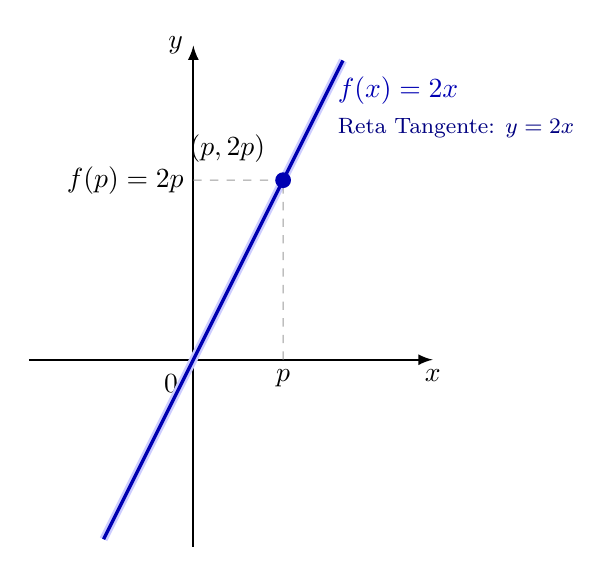
\begin{tikzpicture}[>=latex, scale=0.95]
    \draw[->, thick] (-2.2, 0) -- (3.2, 0) node[below] {$x$};
    \draw[->, thick] (0, -2.5) -- (0, 4.2) node[left] {$y$};
    \node[below left=2pt] at (0, 0) {$0$};

    \draw[line width=3pt, blue!20] (-1.2, -2.4) -- (2.0, 4.0);
    \draw[line width=1.2pt, blue!70!black] (-1.2, -2.4) -- (2.0, 4.0);

    \coordinate (P) at (1.2, 2.4);
    \draw[dashed, gray!80] (1.2, 0) node[below, black] {$p$} -- (P);
    \draw[dashed, gray!80] (0, 2.4) node[left, black] {$f(p) = 2p$} -- (P);

    \fill[blue!70!black] (P) circle (3pt);
    \node[above left=3pt] at (P) {$(p, 2p)$};

    \node[right, blue!70!black] at (1.8, 3.6) {$f(x) = 2x$};
    \node[right, blue!50!black] at (1.8, 3.1) {\footnotesize Reta Tangente: $y = 2x$};
\end{tikzpicture}
\end{center}

\vspace{0.6cm}
\noindent\textbf{Resolução do Exercício 3.}
\label{res:7.2.3}
\linkenunciado{7.2.3}
\setcounter{equation}{0}

\textbf{Determinação da Derivada Geral em um Ponto $p \in \R$:}

Pela definição formal de derivada num ponto arbitrário $p$:
\begin{equation}
    f'(p) = \lim_{x \to p} \frac{f(x) - f(p)}{x - p} \label{eq:def_ex3}
\end{equation}

Para $x \neq p$, manipulamos algebricamente o quociente incremental:
\begin{equation}
    \frac{f(x) - f(p)}{x - p} \label{eq:quociente_ex3}
\end{equation}

Como $f(x) = 3x + 2$, temos $f(p) = 3p + 2$. Substituindo em \eqref{eq:quociente_ex3}:
\begin{align*}
    \frac{f(x) - f(p)}{x - p} &= \frac{(3x + 2) - (3p + 2)}{x - p} \\[0.25cm]
    &= \frac{3x - 3p}{x - p} \\[0.25cm]
    &= \frac{3(x - p)}{x - p} \\[0.25cm]
    &= 3
\end{align*}

Aplicando o limite em \eqref{eq:def_ex3} quando $x \to p$:
\[
f'(p) = \lim_{x \to p} 3 = 3
\]
Como $p$ é um elemento arbitrário do domínio $\R$, concluímos que a derivada é constante e independe do ponto escolhido:
\begin{equation}
    f'(p) = 3 \quad \forall p \in \R \label{eq:resultado_geral_ex3}
\end{equation}

\vspace{0.3cm}
\textbf{Resolução dos Itens por Substituição Direta:}

\begin{enumerate}[label=\alph*)]
    \item $f'(2)$
    
    Fazendo $p = 2$ no resultado geral \eqref{eq:resultado_geral_ex3}:
    \[
    f'(2) = 3 \qedsymbolmath
    \]

    \item $f'(0)$
    
    Fazendo $p = 0$ no resultado geral \eqref{eq:resultado_geral_ex3}:
    \[
    f'(0) = 3 \qedsymbolmath
    \]

    \item $f'(x)$
    
    Sendo a variável independente indicada por $x$, a função derivada associa a cada ponto $x \in \R$ o valor de sua derivada obtido em \eqref{eq:resultado_geral_ex3}:
    \[
    f'(x) = 3 \qedsymbolmath
    \]
\end{enumerate}

\vspace{0.6cm}
\noindent\textbf{Resolução do Exercício 4.}
\label{res:7.2.4}
\linkenunciado{7.2.4}
\setcounter{equation}{0}


\vspace{0.4cm}
\textbf{Resoluções Passo a Passo:}

\begin{enumerate}[label=\alph*)]
    % Item a
    \item $f(x) = x^2 + x$ e $p = 1$

    Calculando o valor de $f$ em $p = 1$:
    \[
    f(1) = 1^2 + 1 = 2
    \]
    Para $x \neq 1$, simplificamos o quociente incremental:
    \begin{align*}
        \frac{f(x) - f(1)}{x - 1} &= \frac{x^2 + x - 2}{x - 1} \\[0.25cm]
        &= \frac{(x - 1)(x + 2)}{x - 1} \\[0.25cm]
        &= x + 2
    \end{align*}
    Calculando o limite pela definição:
    \[
    f'(1) = \lim_{x \to 1} (x + 2) = 1 + 2 = 3
    \]
    \[
    f'(1) = 3 \qedsymbolmath
    \]

    % Item b
    \item $f(x) = \sqrt{x}$ e $p = 4$

    Calculando o valor de $f$ em $p = 4$:
    \[
    f(4) = \sqrt{4} = 2
    \]
    Para $x \neq 4$ com $x \ge 0$, multiplicamos numerador e denominador pelo conjugado $(\sqrt{x} + 2)$:
    \begin{align*}
        \frac{f(x) - f(4)}{x - 4} &= \frac{\sqrt{x} - 2}{x - 4} \\[0.25cm]
        &= \frac{(\sqrt{x} - 2)(\sqrt{x} + 2)}{(x - 4)(\sqrt{x} + 2)} \\[0.25cm]
        &= \frac{x - 4}{(x - 4)(\sqrt{x} + 2)} \\[0.25cm]
        &= \frac{1}{\sqrt{x} + 2}
    \end{align*}
    Passando ao limite quando $x \to 4$:
    \[
    f'(4) = \lim_{x \to 4} \frac{1}{\sqrt{x} + 2} = \frac{1}{\sqrt{4} + 2} = \frac{1}{4}
    \]
    \[
    f'(4) = \frac{1}{4} \qedsymbolmath
    \]

    % Item c
    \item $f(x) = 5x - 3$ e $p = -3$

    Calculando o valor de $f$ em $p = -3$:
    \[
    f(-3) = 5(-3) - 3 = -18
    \]
    Para $x \neq -3$:
    \begin{align*}
        \frac{f(x) - f(-3)}{x - (-3)} &= \frac{(5x - 3) - (-18)}{x + 3} \\[0.25cm]
        &= \frac{5x + 15}{x + 3} \\[0.25cm]
        &= \frac{5(x + 3)}{x + 3} = 5
    \end{align*}
    Passando ao limite quando $x \to -3$:
    \[
    f'(-3) = \lim_{x \to -3} 5 = 5
    \]
    \[
    f'(-3) = 5 \qedsymbolmath
    \]

    % Item d
    \item $f(x) = \dfrac{1}{x}$ e $p = 1$

    Calculando o valor de $f$ em $p = 1$:
    \[
    f(1) = \frac{1}{1} = 1
    \]
    Para $x \neq 1$ e $x \neq 0$:
    \begin{align*}
        \frac{f(x) - f(1)}{x - 1} &= \frac{\dfrac{1}{x} - 1}{x - 1} \\[0.25cm]
        &= \frac{\dfrac{1 - x}{x}}{x - 1} \\[0.25cm]
        &= \frac{-(x - 1)}{x(x - 1)} \\[0.25cm]
        &= -\frac{1}{x}
    \end{align*}
    Passando ao limite quando $x \to 1$:
    \[
    f'(1) = \lim_{x \to 1} \left(-\frac{1}{x}\right) = -1
    \]
    \[
    f'(1) = -1 \qedsymbolmath
    \]

    % Item e
    \item $f(x) = \sqrt{x}$ e $p = 3$

    Calculando o valor de $f$ em $p = 3$:
    \[
    f(3) = \sqrt{3}
    \]
    Para $x \neq 3$ e $x \ge 0$, multiplicamos pelo conjugado $(\sqrt{x} + \sqrt{3})$:
    \begin{align*}
        \frac{f(x) - f(3)}{x - 3} &= \frac{\sqrt{x} - \sqrt{3}}{x - 3} \\[0.25cm]
        &= \frac{(\sqrt{x} - \sqrt{3})(\sqrt{x} + \sqrt{3})}{(x - 3)(\sqrt{x} + \sqrt{3})} \\[0.25cm]
        &= \frac{x - 3}{(x - 3)(\sqrt{x} + \sqrt{3})} \\[0.25cm]
        &= \frac{1}{\sqrt{x} + \sqrt{3}}
    \end{align*}
    Passando ao limite quando $x \to 3$:
    \[
    f'(3) = \lim_{x \to 3} \frac{1}{\sqrt{x} + \sqrt{3}} = \frac{1}{\sqrt{3} + \sqrt{3}} = \frac{1}{2\sqrt{3}} = \frac{\sqrt{3}}{6}
    \]
    \[
    f'(3) = \frac{\sqrt{3}}{6} \qedsymbolmath
    \]

    % Item f
    \item $f(x) = \dfrac{1}{x^2}$ e $p = 2$

    Calculando o valor de $f$ em $p = 2$:
    \[
    f(2) = \frac{1}{2^2} = \frac{1}{4}
    \]
    Para $x \neq 2$ e $x \neq 0$:
    \begin{align*}
        \frac{f(x) - f(2)}{x - 2} &= \frac{\dfrac{1}{x^2} - \dfrac{1}{4}}{x - 2} \\[0.25cm]
        &= \frac{\dfrac{4 - x^2}{4x^2}}{x - 2} \\[0.25cm]
        &= \frac{-(x - 2)(x + 2)}{4x^2(x - 2)} \\[0.25cm]
        &= -\frac{x + 2}{4x^2}
    \end{align*}
    Passando ao limite quando $x \to 2$:
    \[
    f'(2) = \lim_{x \to 2} \left(-\frac{x + 2}{4x^2}\right) = -\frac{2 + 2}{4(2^2)} = -\frac{4}{16} = -\frac{1}{4}
    \]
    \[
    f'(2) = -\frac{1}{4} \qedsymbolmath
    \]

    % Item g
    \item $f(x) = 2x^3 - x^2$ e $p = 1$

    Calculando o valor de $f$ em $p = 1$:
    \[
    f(1) = 2(1)^3 - 1^2 = 1
    \]
    Para $x \neq 1$, manipulamos o quociente incremental:
    \[
    \frac{f(x) - f(1)}{x - 1} = \frac{2x^3 - x^2 - 1}{x - 1}
    \]
    Fatorando o polinômio do numerador $2x^3 - x^2 - 1$ por $(x - 1)$:
    \[
    2x^3 - x^2 - 1 = (x - 1)(2x^2 + x + 1)
    \]
    Portanto:
    \begin{align*}
        \frac{f(x) - f(1)}{x - 1} &= \frac{(x - 1)(2x^2 + x + 1)}{x - 1} = 2x^2 + x + 1
    \end{align*}
    Passando ao limite quando $x \to 1$:
    \[
    f'(1) = \lim_{x \to 1} (2x^2 + x + 1) = 2(1)^2 + 1 + 1 = 4
    \]
    \[
    f'(1) = 4 \qedsymbolmath
    \]

    % Item h
    \item $f(x) = \sqrt[3]{x}$ e $p = 2$

    Calculando o valor de $f$ em $p = 2$:
    \[
    f(2) = \sqrt[3]{2}
    \]
    Para $x \neq 2$:
    \[
    \frac{f(x) - f(2)}{x - 2} = \frac{\sqrt[3]{x} - \sqrt[3]{2}}{x - 2}
    \]
    Utilizando a identidade algébrica da diferença de cubos $A - B = (\sqrt[3]{A} - \sqrt[3]{B})\left(\sqrt[3]{A^2} + \sqrt[3]{AB} + \sqrt[3]{B^2}\right)$ no denominador para simplificar o fator $(\sqrt[3]{x} - \sqrt[3]{2})$:
    \begin{align*}
        \frac{f(x) - f(2)}{x - 2} &= \frac{\sqrt[3]{x} - \sqrt[3]{2}}{(\sqrt[3]{x} - \sqrt[3]{2})\left(\sqrt[3]{x^2} + \sqrt[3]{2x} + \sqrt[3]{4}\right)} \\[0.25cm]
        &= \frac{1}{\sqrt[3]{x^2} + \sqrt[3]{2x} + \sqrt[3]{4}}
    \end{align*}
    Passando ao limite quando $x \to 2$:
    \[
    f'(2) = \lim_{x \to 2} \frac{1}{\sqrt[3]{x^2} + \sqrt[3]{2x} + \sqrt[3]{4}} = \frac{1}{\sqrt[3]{4} + \sqrt[3]{4} + \sqrt[3]{4}} = \frac{1}{3\sqrt[3]{4}} = \frac{\sqrt[3]{2}}{6}
    \]
    \[
    f'(2) = \frac{\sqrt[3]{2}}{6} \qedsymbolmath
    \]
\end{enumerate}

\vspace{0.6cm}
\noindent\textbf{Resolução do Exercício 5.}
\label{res:7.2.5}
\linkenunciado{7.2.5}
\setcounter{equation}{0}

\begin{estrategiabox}[title=Estratégia Geral]
  \begin{itemize}[noitemsep, topsep=2pt]
    \item \textbf{Passo 1:} Determinar o ponto de tangência $(p, f(p))$.
    \item \textbf{Passo 2:} Calcular o coeficiente angular $f'(p)$ pela definição \[\equdefderivadaII\]
    \item \textbf{Passo 3:} Substituir $(p, f(p))$ e $f'(p)$ em \[\equdefretatangente\] e simplificar para a forma reduzida $y = mx + b$.
  \end{itemize}
\end{estrategiabox}

\vspace{0.4cm}
\begin{enumerate}[label=\alph*)]
    % Item a
    \item $f(x) = x^2$ e $p = 2$
    
    \textbf{Passo 1: Determinar o ponto de tangência.}
    \[
    f(2) = 2^2 = 4 \implies (p, f(p)) = (2, 4)
    \]

    \textbf{Passo 2: Calcular o coeficiente angular $f'(2)$ pela definição.}
    Para $x \neq 2$:
    \begin{align*}
        \frac{f(x) - f(2)}{x - 2} &= \frac{x^2 - 4}{x - 2} \\[0.25cm]
        &= \frac{(x - 2)(x + 2)}{x - 2} \\[0.25cm]
        &= x + 2
    \end{align*}
    Passando ao limite quando $x \to 2$:
    \[
    f'(2) = \lim_{x \to 2} (x + 2) = 2 + 2 = 4
    \]

    \textbf{Passo 3: Equação da reta tangente.}

    Substituindo $(p, f(p)) = (2, 4)$ e $f'(2) = 4$:
    \begin{align*}
        y - 4 &= 4(x - 2) \\[0.25cm]
        y - 4 &= 4x - 8 \\[0.25cm]
        y &= 4x - 4
    \end{align*}

    Portanto:
    \[
    y = 4x - 4 \qedsymbolmath
    \]

    % Item b
    \item $f(x) = \dfrac{1}{x}$ e $p = 2$
    
    \textbf{Passo 1: Determinar o ponto de tangência.}
    \[
    f(2) = \frac{1}{2} \implies (p, f(p)) = \left(2, \frac{1}{2}\right)
    \]

    \textbf{Passo 2: Calcular o coeficiente angular $f'(2)$ pela definição.}

    Para $x \neq 2$ e $x \neq 0$:
    \begin{align*}
        \frac{f(x) - f(2)}{x - 2} &= \frac{\dfrac{1}{x} - \dfrac{1}{2}}{x - 2} \\[0.25cm]
        &= \frac{\dfrac{2 - x}{2x}}{x - 2} \\[0.25cm]
        &= \frac{-(x - 2)}{2x(x - 2)} \\[0.25cm]
        &= -\frac{1}{2x}
    \end{align*}
    Passando ao limite quando $x \to 2$:
    \[
    f'(2) = \lim_{x \to 2} \left(-\frac{1}{2x}\right) = -\frac{1}{2(2)} = -\frac{1}{4}
    \]

    \textbf{Passo 3: Equação da reta tangente.}

    Substituindo $(p, f(p)) = \left(2, \dfrac{1}{2}\right)$ e $f'(2) = -\dfrac{1}{4}$:
    \begin{align*}
        y - \frac{1}{2} &= -\frac{1}{4}(x - 2) \\[0.25cm]
        y - \frac{1}{2} &= -\frac{1}{4}x + \frac{1}{2} \\[0.25cm]
        y &= -\frac{1}{4}x + 1
    \end{align*}

    Portanto:
    \[
    y = -\frac{1}{4}x + 1 \qedsymbolmath
    \]

    % Item c
    \item $f(x) = \sqrt{x}$ e $p = 9$
    
    \textbf{Passo 1: Determinar o ponto de tangência.}
    \[
    f(9) = \sqrt{9} = 3 \implies (p, f(p)) = (9, 3)
    \]

    \textbf{Passo 2: Calcular o coeficiente angular $f'(9)$ pela definição.}

    Para $x \neq 9$ com $x \ge 0$, multiplicamos pelo conjugado $(\sqrt{x} + 3)$:
    \begin{align*}
        \frac{f(x) - f(9)}{x - 9} &= \frac{\sqrt{x} - 3}{x - 9} \\[0.25cm]
        &= \frac{(\sqrt{x} - 3)(\sqrt{x} + 3)}{(x - 9)(\sqrt{x} + 3)} \\[0.25cm]
        &= \frac{x - 9}{(x - 9)(\sqrt{x} + 3)} \\[0.25cm]
        &= \frac{1}{\sqrt{x} + 3}
    \end{align*}
    Passando ao limite quando $x \to 9$:
    \[
    f'(9) = \lim_{x \to 9} \frac{1}{\sqrt{x} + 3} = \frac{1}{\sqrt{9} + 3} = \frac{1}{6}
    \]

    \textbf{Passo 3: Equação da reta tangente.}

    Substituindo $(p, f(p)) = (9, 3)$ e $f'(9) = \dfrac{1}{6}$:
    \begin{align*}
        y - 3 &= \frac{1}{6}(x - 9) \\[0.25cm]
        y - 3 &= \frac{1}{6}x - \frac{3}{2} \\[0.25cm]
        y &= \frac{1}{6}x + \frac{3}{2}
    \end{align*}

    Portanto:
    \[
    y = \frac{1}{6}x + \frac{3}{2} \qedsymbolmath
    \]

    % Item d
    \item $f(x) = x^2 - x$ e $p = 1$
    
    \textbf{Passo 1: Determinar o ponto de tangência.}
    \[
    f(1) = 1^2 - 1 = 0 \implies (p, f(p)) = (1, 0)
    \]

    \textbf{Passo 2: Calcular o coeficiente angular $f'(1)$ pela definição.}

    Para $x \neq 1$:
    \begin{align*}
        \frac{f(x) - f(1)}{x - 1} &= \frac{(x^2 - x) - 0}{x - 1} \\[0.25cm]
        &= \frac{x(x - 1)}{x - 1} \\[0.25cm]
        &= x
    \end{align*}
    Passando ao limite quando $x \to 1$:
    \[
    f'(1) = \lim_{x \to 1} x = 1
    \]

    \textbf{Passo 3: Equação da reta tangente.}

    Substituindo $(p, f(p)) = (1, 0)$ e $f'(1) = 1$:
    \begin{align*}
        y - 0 &= 1(x - 1) \\[0.25cm]
        y &= x - 1
    \end{align*}

    Portanto:
    \[
    y = x - 1 \qedsymbolmath
    \]
\end{enumerate}

\vspace{0.6cm}
\noindent\textbf{Resolução do Exercício 6.}
\label{res:7.2.6}
\linkenunciado{7.2.6}
\setcounter{equation}{0}

\begin{estrategiabox}[title=Estratégia Geral de Resolução]
  \begin{itemize}[noitemsep, topsep=2pt]
    \item \textbf{Passo 1:} Montar o quociente incremental usando a definição por acréscimo avaliada no ponto genérico $x$.
    \item \textbf{Passo 2:} Expandir os termos quadráticos e lineares de $f(x + h)$ e cancelar os termos correspondentes a $f(x)$.
    \item \textbf{Passo 3:} Fatorar o acréscimo $h$ do numerador para cancelar a indeterminação $\left[\frac{0}{0}\right]$ e aplicar a passagem direta ao limite quando $h \to 0$.
  \end{itemize}
\end{estrategiabox}

\paragraph{a) $f(x) = x^2 + x$}

Pela definição por acréscimo no ponto $x$, temos:
\begin{equation}
f'(x) = \lim_{h \to 0} \frac{f(x + h) - f(x)}{h} \label{eq:res_6_a_def}
\end{equation}

Substituindo $f(x + h) = (x + h)^2 + (x + h)$ e $f(x) = x^2 + x$ no numerador:
\begin{align*}
f(x + h) - f(x) &= \left[(x + h)^2 + (x + h)\right] - (x^2 + x) \\
&= \left(x^2 + 2xh + h^2 + x + h\right) - x^2 - x \\
&= 2xh + h^2 + h
\end{align*}

Inserindo o numerador simplificado no quociente incremental da equação \eqref{eq:res_6_a_def}:
\begin{align*}
f'(x) &= \lim_{h \to 0} \frac{2xh + h^2 + h}{h} \\
      &= \lim_{h \to 0} \frac{h(2x + h + 1)}{h} \\
      &= \lim_{h \to 0} (2x + h + 1) \\
      &= 2x + 0 + 1 \\
      &= 2x + 1
\end{align*}

Portanto:
\[
  f'(x) = 2x + 1 \qedsymbolmath
\]

\setcounter{equation}{0}
\paragraph{b) $f(x) = 3x - 1$}

Pela definição por acréscimo no ponto $x$, temos:
\begin{equation}
f'(x) = \lim_{h \to 0} \frac{f(x + h) - f(x)}{h} \label{eq:res_6_b_def}
\end{equation}

Substituindo $f(x + h) = 3(x + h) - 1$ e $f(x) = 3x - 1$ no numerador:
\begin{align*}
f(x + h) - f(x) &= [3(x + h) - 1] - (3x - 1) \\
&= (3x + 3h - 1) - 3x + 1 \\
&= 3h
\end{align*}

Inserindo o numerador simplificado no quociente incremental da equação \eqref{eq:res_6_b_def}:
\begin{align*}
f'(x) &= \lim_{h \to 0} \frac{3h}{h} \\
      &= \lim_{h \to 0} 3 \\
      &= 3
\end{align*}

Portanto:
\[
  f'(x) = 3 \qedsymbolmath
\]

\setcounter{equation}{0}
\paragraph{c) $f(x) = x^3$}

Pela definição por acréscimo no ponto $x$, temos:
\begin{equation}
f'(x) = \lim_{h \to 0} \frac{f(x + h) - f(x)}{h} \label{eq:res_6_c_def}
\end{equation}

Substituindo $f(x + h) = (x + h)^3$ e $f(x) = x^3$ no numerador:
\begin{align*}
f(x + h) - f(x) &= (x + h)^3 - x^3 \\
&= (x^3 + 3x^2h + 3xh^2 + h^3) - x^3 \\
&= 3x^2h + 3xh^2 + h^3
\end{align*}

Inserindo o numerador simplificado no quociente incremental da equação \eqref{eq:res_6_c_def}:
\begin{align*}
f'(x) &= \lim_{h \to 0} \frac{3x^2h + 3xh^2 + h^3}{h} \\
      &= \lim_{h \to 0} \frac{h(3x^2 + 3xh + h^2)}{h} \\
      &= \lim_{h \to 0} (3x^2 + 3xh + h^2) \\
      &= 3x^2 + 3x(0) + 0^2 \\
      &= 3x^2
\end{align*}

Portanto:
\[
  f'(x) = 3x^2 \qedsymbolmath
\]

\setcounter{equation}{0}
\paragraph{d) $f(x) = \frac{1}{x}$}

Pela definição por acréscimo no ponto $x$, temos:
\begin{equation}
f'(x) = \lim_{h \to 0} \frac{f(x + h) - f(x)}{h} \label{eq:res_6_d_def}
\end{equation}

Substituindo $f(x + h) = \frac{1}{x + h}$ e $f(x) = \frac{1}{x}$ no numerador:
\begin{align*}
f(x + h) - f(x) &= \frac{1}{x + h} - \frac{1}{x} \\
&= \frac{x - (x + h)}{x(x + h)} \\
&= \frac{-h}{x(x + h)}
\end{align*}

Inserindo o numerador simplificado no quociente incremental da equação \eqref{eq:res_6_d_def}:
\begin{align*}
f'(x) &= \lim_{h \to 0} \frac{\frac{-h}{x(x + h)}}{h} \\
      &= \lim_{h \to 0} \left[ \frac{-h}{x(x + h)} \cdot \frac{1}{h} \right] \\
      &= \lim_{h \to 0} \frac{-1}{x(x + h)} \\
      &= \frac{-1}{x(x + 0)} \\
      &= -\frac{1}{x^2}
\end{align*}

Portanto:
\[
  f'(x) = -\frac{1}{x^2} \qedsymbolmath
\]

\setcounter{equation}{0}
\paragraph{e) $f(x) = 5x$}

Pela definição por acréscimo no ponto $x$, temos:
\begin{equation}
f'(x) = \lim_{h \to 0} \frac{f(x + h) - f(x)}{h} \label{eq:res_6_e_def}
\end{equation}

Substituindo $f(x + h) = 5(x + h)$ e $f(x) = 5x$ no numerador:
\begin{align*}
f(x + h) - f(x) &= 5(x + h) - 5x \\
&= 5x + 5h - 5x \\
&= 5h
\end{align*}

Inserindo o numerador simplificado no quociente incremental da equação \eqref{eq:res_6_e_def}:
\begin{align*}
f'(x) &= \lim_{h \to 0} \frac{5h}{h} \\
      &= \lim_{h \to 0} 5 \\
      &= 5
\end{align*}

Portanto:
\[
  f'(x) = 5 \qedsymbolmath
\]

\setcounter{equation}{0}
\paragraph{f) $f(x) = 10$}

Pela definição por acréscimo no ponto $x$, temos:
\begin{equation}
f'(x) = \lim_{h \to 0} \frac{f(x + h) - f(x)}{h} \label{eq:res_6_f_def}
\end{equation}

Como $f$ é uma função constante, $f(x + h) = 10$ e $f(x) = 10$ para qualquer valor de entrada:
\begin{align*}
f(x + h) - f(x) &= 10 - 10 \\
&= 0
\end{align*}

Inserindo no quociente incremental da equação \eqref{eq:res_6_f_def}:
\begin{align*}
f'(x) &= \lim_{h \to 0} \frac{0}{h} \\
      &= \lim_{h \to 0} 0 \\
      &= 0
\end{align*}

Portanto:
\[
  f'(x) = 0 \qedsymbolmath
\]

\setcounter{equation}{0}
\paragraph{g) $f(x) = \frac{x}{x + 1}$}

Pela definição por acréscimo no ponto $x$, temos:
\begin{equation}
f'(x) = \lim_{h \to 0} \frac{f(x + h) - f(x)}{h} \label{eq:res_6_g_def}
\end{equation}

Substituindo $f(x + h) = \frac{x + h}{(x + h) + 1}$ e $f(x) = \frac{x}{x + 1}$ no numerador:
\begin{align*}
f(x + h) - f(x) &= \frac{x + h}{x + h + 1} - \frac{x}{x + 1} \\
&= \frac{(x + h)(x + 1) - x(x + h + 1)}{(x + h + 1)(x + 1)} \\
&= \frac{(x^2 + x + hx + h) - (x^2 + xh + x)}{(x + h + 1)(x + 1)} \\
&= \frac{h}{(x + h + 1)(x + 1)}
\end{align*}

Inserindo o numerador simplificado no quociente incremental da equação \eqref{eq:res_6_g_def}:
\begin{align*}
f'(x) &= \lim_{h \to 0} \frac{\frac{h}{(x + h + 1)(x + 1)}}{h} \\
      &= \lim_{h \to 0} \left[ \frac{h}{(x + h + 1)(x + 1)} \cdot \frac{1}{h} \right] \\
      &= \lim_{h \to 0} \frac{1}{(x + h + 1)(x + 1)} \\
      &= \frac{1}{(x + 0 + 1)(x + 1)} \\
      &= \frac{1}{(x + 1)^2}
\end{align*}

Portanto:
\[
  f'(x) = \frac{1}{(x + 1)^2} \qedsymbolmath
\]

\setcounter{equation}{0}
\paragraph{h) $f(x) = \frac{1}{x^2}$}

Pela definição por acréscimo no ponto $x$, temos:
\begin{equation}
f'(x) = \lim_{h \to 0} \frac{f(x + h) - f(x)}{h} \label{eq:res_6_h_def}
\end{equation}

Substituindo $f(x + h) = \frac{1}{(x + h)^2}$ e $f(x) = \frac{1}{x^2}$ no numerador:
\begin{align*}
f(x + h) - f(x) &= \frac{1}{(x + h)^2} - \frac{1}{x^2} \\
&= \frac{x^2 - (x + h)^2}{x^2(x + h)^2} \\
&= \frac{x^2 - (x^2 + 2xh + h^2)}{x^2(x + h)^2} \\
&= \frac{-2xh - h^2}{x^2(x + h)^2} \\
&= \frac{-h(2x + h)}{x^2(x + h)^2}
\end{align*}

Inserindo o numerador simplificado no quociente incremental da equação \eqref{eq:res_6_h_def}:
\begin{align*}
f'(x) &= \lim_{h \to 0} \frac{\frac{-h(2x + h)}{x^2(x + h)^2}}{h} \\
      &= \lim_{h \to 0} \left[ \frac{-h(2x + h)}{x^2(x + h)^2} \cdot \frac{1}{h} \right] \\
      &= \lim_{h \to 0} \frac{-(2x + h)}{x^2(x + h)^2} \\
      &= \frac{-(2x + 0)}{x^2(x + 0)^2} \\
      &= \frac{-2x}{x^4} \\
      &= -\frac{2}{x^3}
\end{align*}

Portanto:
\[
  f'(x) = -\frac{2}{x^3} \qedsymbolmath
\]
% ------------------------------------------------------------------------------
% 7.3 a 7.17 (ESTRUTURA DE ESPERA PARA PRÓXIMAS RESOLUÇÕES)
% ------------------------------------------------------------------------------
\subsection*{7.3. Derivadas de $x^n$ e $\sqrt[n]{x}$}
\subsection*{7.4. Derivadas de $e^x$ e $\ln(x)$}
\subsection*{7.5. Derivadas de Funções Trigonométricas}
\subsection*{7.6. Derivabilidade e Continuidade}
\subsection*{7.7. Regras de Derivação}
\subsection*{7.8. Função Derivada e Derivadas de Ordem Superior}
\subsection*{7.9. Notações para a Derivada}
\subsection*{7.10. Regra da Cadeia para Derivação de Função Composta}
\textit{Esta subseção não possui exercícios.}
\subsection*{7.11. Aplicações da Regra da Cadeia}
\subsection*{7.12. Derivada de $f(x)^{g(x)}$}
\subsection*{7.13. Derivação da Função Dada Implicitamente}
\subsection*{7.14. Interpretação de $\frac{\diff y}{\diff x}$ como um Quociente Diferencial}
\subsection*{7.15. Velocidade e Aceleração. Taxa de Variação}
\subsection*{7.16. Problemas Reta Tangente e Normal ao Gráfico de uma Função}
\subsection*{7.17. Exercícios do Capítulo}
